% =============================================================================
% relatorio_alu.tex -- Relatorio Tecnico: ALUChip v1.0
% Unidade 7 | Capitulo 5 | Desafio de Design de CIs -- PADIS
% Autor  : Romulo da Silva Lira
% Prof.  : Andre Feitosa
% =============================================================================
\documentclass[12pt,a4paper]{article}

\usepackage[utf8]{inputenc}
\usepackage[T1]{fontenc}
\usepackage[brazil]{babel}
\usepackage{lmodern}
\usepackage{microtype}
\usepackage{geometry}
% Margens ABNT (NBR 14724): esq=3cm, dir=2cm, sup=3cm, inf=2cm
\geometry{top=3cm,bottom=2cm,left=3cm,right=2cm}
\usepackage{setspace}
\onehalfspacing   % espacamento 1,5 ABNT
\usepackage{graphicx}
\usepackage[dvipsnames,table]{xcolor}
\usepackage{tikz}
\usetikzlibrary{shapes.geometric,arrows.meta,positioning,fit,calc,shadows,decorations.pathreplacing}
\usepackage{pgfplots}
\pgfplotsset{compat=1.18}
\usepackage{booktabs,multirow,array,longtable,colortbl}
\usepackage{listings,caption,subcaption}
\usepackage{amsmath,amssymb,mathtools,bm}
\usepackage{fancyhdr,titlesec,setspace,parskip,enumitem}
\usepackage[most]{tcolorbox}
\tcbuselibrary{listings,breakable,skins}
\usepackage[hidelinks,pdftitle={ALUChip v1.0},pdfauthor={Romulo da Silva Lira}]{hyperref}
\usepackage{siunitx}
\sisetup{output-decimal-marker={,},group-separator={.}}

% ── Cores ────────────────────────────────────────────────────────────────────
\definecolor{alublue}{RGB}{21,101,192}
\definecolor{aluteal}{RGB}{0,137,123}
\definecolor{alured}{RGB}{198,40,40}
\definecolor{alugreen}{RGB}{46,125,50}
\definecolor{aluorange}{RGB}{239,108,0}
\definecolor{alugray}{RGB}{66,66,66}
\definecolor{alubg}{RGB}{245,248,252}
\definecolor{alucode}{RGB}{248,248,248}

% ── Listagem SV ──────────────────────────────────────────────────────────────
\lstdefinelanguage{SystemVerilog}{
  morekeywords={module,endmodule,input,output,logic,wire,reg,always_comb,
    assign,begin,end,case,endcase,default,if,else,parameter,localparam,
    task,endtask,automatic,initial,$dumpfile,$dumpvars,$display,$finish,int,
    timescale,string},
  sensitive=true,
  morecomment=[l]{//},
  morestring=[b]",
}
\lstdefinestyle{svstyle}{
  language=SystemVerilog,
  basicstyle=\ttfamily\small,
  keywordstyle=\color{alublue}\bfseries,
  commentstyle=\color{alugray}\itshape,
  numbers=left, numberstyle=\tiny\color{alugray}, stepnumber=1, numbersep=8pt,
  frame=single, framerule=0.6pt, rulecolor=\color{alublue!40},
  backgroundcolor=\color{alucode},
  breaklines=true, showstringspaces=false, tabsize=4, captionpos=b,
  xleftmargin=15pt, xrightmargin=5pt,
}

% ── Caixas ───────────────────────────────────────────────────────────────────
\newtcolorbox{unidadebox}[1][]{enhanced,colback=alubg,colframe=alublue,
  coltitle=white,fonttitle=\bfseries\normalsize,title={#1},boxrule=1.2pt,
  arc=4pt,left=8pt,right=8pt,top=6pt,bottom=6pt,
  shadow={2pt}{-2pt}{0pt}{black!20},breakable}
\newtcolorbox{resultbox}[1][]{enhanced,colback=alugreen!5,
  colframe=alugreen!70!black,coltitle=white,fonttitle=\bfseries\small,
  title={#1},boxrule=1pt,arc=3pt,left=6pt,right=6pt,top=5pt,bottom=5pt,breakable}
\newtcolorbox{specbox}[1][]{enhanced,colback=alublue!5,colframe=alublue!60,
  coltitle=alublue!80!black,fonttitle=\bfseries\small,title={#1},
  boxrule=0.8pt,arc=3pt,left=6pt,right=6pt,top=5pt,bottom=5pt,breakable}

% ── Cabecalho ────────────────────────────────────────────────────────────────
\pagestyle{fancy}\fancyhf{}
\fancyhead[L]{\small\textcolor{alublue}{\textbf{ALUChip v1.0}} \textcolor{alugray}{--- ULA 8 bits}}
\fancyhead[R]{\small\textcolor{alugray}{PADIS $|$ Unidade~7 $|$ Cap.~5}}
\fancyfoot[L]{\small\textcolor{alugray}{Rômulo da Silva Lira --- UFAM/ICOMP}}
\fancyfoot[C]{\small\textcolor{alugray}{\thepage}}
\fancyfoot[R]{\small\textcolor{alugray}{Prof.\ André Feitosa}}
\renewcommand{\headrulewidth}{0.6pt}
\renewcommand{\footrulewidth}{0.4pt}
\renewcommand{\headrule}{\hbox to\headwidth{\color{alublue}\leaders\hrule height \headrulewidth\hfill}}

% ── Titulos ──────────────────────────────────────────────────────────────────
\titleformat{\section}{\large\bfseries\color{alublue}}{\thesection.}{0.6em}{}
  [\vspace{-4pt}\textcolor{alublue}{\hrule height 0.6pt}\vspace{2pt}]
\titleformat{\subsection}{\normalsize\bfseries\color{aluteal}}{\thesubsection.}{0.5em}{}
\titleformat{\subsubsection}{\normalsize\bfseries\color{alugray}}{\thesubsubsection.}{0.4em}{}

% =============================================================================
\begin{document}
\thispagestyle{empty}

% ── Capa UFAM (NBR 14724) ────────────────────────────────────────────────────
\begin{center}
  \vspace*{0.5cm}
  {\normalsize\bfseries UNIVERSIDADE FEDERAL DO AMAZONAS -- UFAM}\\[3pt]
  {\normalsize\bfseries Instituto de Computação -- ICOMP}\\[3pt]
  {\normalsize Departamento de Engenharia de Computação e Sistemas}\\[3pt]
  {\normalsize Projeto de Análise e Design de Sistemas Integrados -- PADIS}\\[40pt]

  {\LARGE\bfseries\color{alublue} ALUChip v1.0}\\[10pt]
  {\large\bfseries Unidade Lógico-Aritmética de 8~Bits}\\[6pt]
  {\normalsize\color{alugray}
    8~Operações $|$ 4~\textit{Flags} $|$ CMOS 0,35\,\textmu m $|$ VDD\,=\,3,3\,V}\\[40pt]

  {\normalsize\bfseries Rômulo da Silva Lira}\\[60pt]

  \vfill
  {\normalsize\textbf{Orientador:} Prof.\ André Feitosa}\\[6pt]
  {\normalsize Unidade~7 --- Capítulo~5 | Desafio de Design de Circuitos Integrados}\\[6pt]
  {\normalsize Manaus -- AM}\\[4pt]
  {\normalsize \the\year}
\end{center}

\newpage
\thispagestyle{empty}
\begin{center}
  \vspace*{0.5cm}
  {\normalsize\bfseries UNIVERSIDADE FEDERAL DO AMAZONAS -- UFAM}\\[3pt]
  {\normalsize\bfseries Instituto de Computação -- ICOMP}\\[30pt]

  {\normalsize\bfseries Rômulo da Silva Lira}\\[40pt]

  {\LARGE\bfseries\color{alublue} ALUChip v1.0}\\[10pt]
  {\large\bfseries Unidade Lógico-Aritmética de 8~Bits}\\[40pt]

  \begin{minipage}{0.55\textwidth}
  \begin{flushright}
    {\small Trabalho apresentado à disciplina Projeto de Análise e Design de Sistemas Integrados -- PADIS, como requisito parcial para conclusão do Desafio de Design de Circuitos Integrados.}\\[10pt]
    {\small \textbf{Orientador:} Prof.\ André Feitosa}
  \end{flushright}
  \end{minipage}\\[60pt]

  \vfill
  {\normalsize Manaus -- AM}\\[4pt]
  {\normalsize \the\year}
\end{center}

\newpage\thispagestyle{empty}\vspace*{3cm}
\begin{center}
  \begin{tabular}{rl}
    \textbf{Autor:}      & Rômulo da Silva Lira \\
    \textbf{Professor:}  & André Feitosa \\
    \textbf{Instituição:}& UFAM --- Instituto de Computação \\
    \textbf{Disciplina:} & PADIS --- Unidade~7, Capítulo~5 \\
    \textbf{Entrega:}    & Desafio de Design de Circuitos Integrados \\
    \textbf{Data:}       & \today \\
  \end{tabular}
\end{center}
\vspace{1cm}
\begin{center}

  \begin{tikzpicture}[
    box/.style={draw=alublue,fill=alubg,rounded corners=4pt,
                minimum width=2.4cm,minimum height=1.1cm,align=center,
                font=\small\bfseries},
    mux/.style={draw=aluorange,fill=aluorange!10,rounded corners=2pt,
                minimum width=1.4cm,minimum height=2.4cm,align=center,
                font=\small\bfseries\color{aluorange}},
    arr/.style={-{Stealth[scale=1.1]},thick}
  ]
    \node[box,fill=alublue!10] (add) at (0,1.2) {Adder\\ADD/SUB};
    \node[box,fill=alugreen!10] (log) at (0,0) {Logic\\AND·OR·XOR·NOT};
    \node[box,fill=aluorange!10] (shf) at (0,-1.2) {Shifter\\SHL·SHR};
    \node[mux] (mux) at (3.2,0) {MUX\\8:1};
    \node[box,fill=alured!10] (flg) at (6.0,0) {Flags\\Z·C·V·N};
    \draw[arr,alublue] (add.east) -- (mux.west|-add.east);
    \draw[arr,alugreen] (log.east) -- (mux.west);
    \draw[arr,aluorange] (shf.east) -- (mux.west|-shf.east);
    \draw[arr,alublue] (mux.east) -- node[above,font=\tiny\ttfamily]{RESULT[7:0]} (flg.west);
    \draw[arr,alured] (flg.east) -- ++(1.2,0) node[right,font=\tiny\ttfamily]{Z C V N};
    \node[left=1.5cm of add,font=\tiny\ttfamily,text=alublue] (ia) {A[7:0]};
    \draw[arr,alublue!60] (ia.east) -- (add.west);
    \draw[arr,alublue!60] (ia.east|-log.west) -- (log.west);
    \draw[arr,alublue!60] (ia.east|-shf.west) -- (shf.west);
    \node[below=0.5cm of mux,font=\tiny\ttfamily,text=aluorange] {OP[2:0]};
    \draw[arr,aluorange!80] (3.2,-0.9) -- (mux.south);
  \end{tikzpicture}

  \vfill
  {\small\textcolor{alugray}{Simulação funcional: \textbf{27/27 testes aprovados} (Icarus Verilog v12)}}
\end{center}

\newpage

% ── Resumo ───────────────────────────────────────────────────────────────────
\begin{center}{\large\bfseries\color{alublue} Resumo}\end{center}
\begin{unidadebox}[Resumo]
Este trabalho descreve o projeto completo do \textbf{ALUChip v1.0}, uma Unidade Lógico-Aritmética (ULA) de 8~bits com 8~operações e 4~flags de estado, implementada em processo CMOS 0,35\,\textmu m com tensão de alimentação de 3,3\,V. O circuito executa operações aritméticas (\texttt{ADD}, \texttt{SUB}), lógicas (\texttt{AND}, \texttt{OR}, \texttt{XOR}, \texttt{NOT}) e de deslocamento (\texttt{SHL}, \texttt{SHR}) selecionadas por um código de 3~bits, produzindo um resultado de 8~bits e quatro sinalizadores: \textit{Zero}~(Z), \textit{Carry}~(C), \textit{Overflow}~(V) e \textit{Negativo}~(N). A lógica é inteiramente combinacional, resultando em latência de propagação estimada em 1,4\,ns no caminho crítico (ADD/SUB). A verificação funcional com Icarus Verilog v12 obteve \textbf{aprovação em 27/27 vetores de teste}, cobrindo todos os 8~grupos de operações e cenários de borda (carry, overflow, zero, negativo). A área de \textit{core} estimada é de $\approx$520\,\textmu m² e o consumo dinâmico de $\approx$32\,\textmu W a 100\,MHz. O ALUChip v1.0 é adequado como núcleo aritmético de microprocessadores de baixo custo, controladores embarcados e sistemas de DSP dedicados.\\[4pt]
\textbf{Palavras-chave:} ULA; ALU; 8~bits; lógica combinacional; CMOS 0,35\,\textmu m; flags; SystemVerilog.
\end{unidadebox}

\vspace{6pt}
\begin{center}{\large\bfseries\color{alublue} Abstract}\end{center}
\begin{unidadebox}[Abstract]
This paper presents the complete design of \textbf{ALUChip v1.0}, an 8-bit Arithmetic Logic Unit (ALU) featuring 8 operations and 4 status flags, targeting a CMOS 0.35\,\textmu m process at 3.3\,V supply. The circuit performs arithmetic (\texttt{ADD}, \texttt{SUB}), logic (\texttt{AND}, \texttt{OR}, \texttt{XOR}, \texttt{NOT}), and shift (\texttt{SHL}, \texttt{SHR}) operations selected by a 3-bit opcode, delivering an 8-bit result and four flags: \textit{Zero}~(Z), \textit{Carry}~(C), \textit{Overflow}~(V), and \textit{Negative}~(N). The all-combinational datapath yields an estimated propagation delay of 1.4\,ns on the critical path (ADD/SUB). Functional verification under Icarus Verilog v12 achieved \textbf{27/27 test-vector pass rate}, covering all 8 operation groups and boundary conditions. Synthesis estimates indicate a core area of $\approx$520\,\textmu m² and dynamic power of $\approx$32\,\textmu W at 100\,MHz. ALUChip v1.0 is suitable as the arithmetic core for low-cost microprocessors, embedded controllers, and dedicated DSP systems.\\[4pt]
\textbf{Keywords:} ALU; 8-bit; combinational logic; CMOS 0.35\,\textmu m; status flags; SystemVerilog.
\end{unidadebox}

\newpage
\tableofcontents
\listoffigures
\listoftables
\newpage

% =============================================================================
\section{Introdução}
% =============================================================================

A Unidade Lógico-Aritmética (ULA, ou \textit{Arithmetic Logic Unit} --- ALU) é o bloco funcional mais fundamental de qualquer processador digital. Proposta na forma moderna por John von Neumann em seu relatório de 1945~\cite{vonneumann1945} e concretizada em silício no Intel 4004 (1971)~\cite{intel4004}, a ALU executa operações matemáticas e lógicas sobre dados binários, produzindo sinalizadores de estado (\textit{flags}) que controlam o fluxo do programa por meio de instruções de desvio condicional.

\begin{unidadebox}[Importância Histórica e Industrial da ALU]
\begin{itemize}[leftmargin=1.5em]
  \item \textbf{Intel 4004 (1971):} primeira ALU de 4~bits em um único CI, 2.300 transistores, processo 10\,\textmu m.
  \item \textbf{Intel 8080 (1974):} ALU de 8~bits, base do CP/M e do MS-DOS; mesmo tamanho de dados do ALUChip v1.0.
  \item \textbf{ARMv7/v8:} ALU de 32/64~bits com suporte a SIMD; toda instrução aritmética passa por um bloco equivalente ao projetado aqui.
  \item \textbf{RISC-V (2010--):} ISA aberta com ALU de 32/64~bits; o conjunto mínimo RV32I usa exatamente ADD, SUB, AND, OR, XOR e deslocamentos --- as mesmas 8~operações do ALUChip v1.0.
\end{itemize}
\end{unidadebox}

O \textbf{ALUChip v1.0} implementa uma ULA de 8~bits com as 8~operações fundamentais do repertório RISC, em processo CMOS 0,35\,\textmu m com 3,3\,V. O design é inteiramente combinacional, garantindo zero latência de pipeline para integração em caminhos de dados críticos de microcontroladores e sistemas embarcados.

% =============================================================================
\section{Objetivos}
% =============================================================================

\subsection{Objetivo Geral}

Projetar, implementar em RTL SystemVerilog e verificar funcionalmente a ULA de 8~bits \textbf{ALUChip v1.0}, demonstrando o fluxo completo de design de circuitos integrados digitais: especificação, codificação RTL, simulação funcional, análise de \textit{timing}, estimativa de área e verificação de \textit{layout}.

\subsection{Objetivos Específicos}

\begin{enumerate}[leftmargin=2em,label=\textbf{O\arabic*.}]
  \item Especificar formalmente as 8~operações da ULA e a semântica das 4~\textit{flags} de estado (Z, C, V, N).
  \item Implementar o núcleo \texttt{alu8} em SystemVerilog IEEE 1800-2012 como lógica puramente combinacional.
  \item Implementar o \textit{top-level} \texttt{alu8\_chip\_top} integrando o núcleo e os pads de I/O.
  \item Verificar o funcionamento por \textit{testbench} abrangente com 27~vetores cobrindo todos os grupos operacionais e condições de borda.
  \item Gerar esquemáticos do somador \textit{Ripple-Carry} e das unidades lógica e de deslocamento.
  \item Estimar \textit{timing}, área de \textit{core} e consumo de potência para o processo CMOS 0,35\,\textmu m.
  \item Avaliar o \textit{floorplan} e as verificações DRC/LVS do \textit{layout} proposto.
\end{enumerate}

% =============================================================================
\section{Materiais e Metodologia}
% =============================================================================

\subsection{Especificação das Operações}

A tabela~\ref{tab:ops} define formalmente as 8~operações implementadas, o código de 3~bits e o comportamento das \textit{flags}.

\begin{table}[h!]
\centering
\caption{Tabela de operações do ALUChip v1.0}
\label{tab:ops}
\rowcolors{2}{alubg}{white}
\begin{tabular}{c c l l l}
\toprule
\textbf{OP[2:0]} & \textbf{Mnemônico} & \textbf{Operação} & \textbf{Flags atualizadas} & \textbf{Aplicação típica} \\
\midrule
\texttt{000} & ADD  & $\text{R} = A + B$         & Z, C, V, N & Adição inteira \\
\texttt{001} & SUB  & $\text{R} = A - B$         & Z, C, V, N & Subtração / comparação \\
\texttt{010} & AND  & $\text{R} = A \land B$     & Z, N       & Máscara de bits \\
\texttt{011} & OR   & $\text{R} = A \lor B$      & Z, N       & Set de bits \\
\texttt{100} & XOR  & $\text{R} = A \oplus B$    & Z, N       & Toggle / comparação \\
\texttt{101} & NOT  & $\text{R} = \overline{A}$  & Z, N       & Inversão (B ignorado) \\
\texttt{110} & SHL  & $\text{R} = A \ll 1,\ C = A_7$ & Z, C, N  & Multiplica por 2 \\
\texttt{111} & SHR  & $\text{R} = A \gg 1,\ C = A_0$ & Z, C, N  & Divide por 2 \\
\bottomrule
\end{tabular}
\end{table}

\subsection{Semântica das Flags}

As 4~\textit{flags} de estado do ALUChip v1.0 são definidas formalmente abaixo:

\begin{align}
  Z &= (R[7:0] = 0\text{x}00)
    \qquad\text{(NOR de todos os 8~bits do resultado)} \label{eq:z}\\
  C &= \text{carry-out}_{[8]} \text{ (ADD/SUB)}
     \;|\; A_7 \text{ (SHL)}
     \;|\; A_0 \text{ (SHR)} \label{eq:c}\\
  V &= (\overline{A_7} \cdot \overline{B_7} \cdot R_7) \lor (A_7 \cdot B_7 \cdot \overline{R_7})
    \quad\text{(ADD); sinal trocado} \label{eq:v}\\
  N &= R[7]
    \qquad\text{(MSB do resultado, indica número negativo em C2)} \label{eq:n}
\end{align}

\subsection{Implementação RTL}

\subsubsection{Núcleo da ULA}

\begin{lstlisting}[style=svstyle,caption={alu8.sv --- Núcleo combinacional da ULA de 8 bits},label=lst:alu]
module alu8 (
    input  logic [7:0] a, b,
    input  logic [2:0] op,
    output logic [7:0] result,
    output logic       flag_z, flag_c, flag_v, flag_n
);
    logic [8:0] wide;

    // Bits extraidos para compatibilidade com Icarus
    logic a_msb, b_msb, a_lsb;
    logic [6:0] a_lo7, a_hi7;
    assign a_msb = a[7];  assign b_msb = b[7];  assign a_lsb = a[0];
    assign a_lo7 = a[6:0];  assign a_hi7 = a[7:1];

    always_comb begin
        case (op)
            3'b000: wide = {1'b0, a} + {1'b0, b};           // ADD
            3'b001: wide = {1'b0, a} + {1'b0, ~b} + 9'd1;  // SUB
            3'b010: wide = {1'b0, a & b};                   // AND
            3'b011: wide = {1'b0, a | b};                   // OR
            3'b100: wide = {1'b0, a ^ b};                   // XOR
            3'b101: wide = {1'b0, ~a};                      // NOT
            3'b110: wide = {a_msb, a_lo7, 1'b0};            // SHL
            3'b111: wide = {a_lsb, 1'b0, a_hi7};            // SHR
            default: wide = 9'b0;
        endcase
    end

    logic res_msb;
    assign res_msb = wide[7];
    assign flag_v  =
        ((op == 3'b000) & ((~a_msb & ~b_msb &  res_msb) |
                           ( a_msb &  b_msb & ~res_msb))) |
        ((op == 3'b001) & ((~a_msb &  b_msb &  res_msb) |
                           ( a_msb & ~b_msb & ~res_msb)));

    assign result = wide[7:0];
    assign flag_c = wide[8];
    assign flag_z = (wide[7:0] == 8'h00);
    assign flag_n = wide[7];
endmodule
\end{lstlisting}

O núcleo é organizado em três caminhos paralelos:
\begin{itemize}[leftmargin=1.5em]
  \item \textbf{Caminho aritmético (ADD/SUB):} Somador de 9~bits utilizando o operador \texttt{+} do SystemVerilog. A subtração é implementada como $A + \overline{B} + 1$ (complemento de 2), permitindo reutilizar o mesmo somador para ambas as operações.
  \item \textbf{Caminho lógico (AND/OR/XOR/NOT):} Operações bit a bit diretas, sem propagação de carry.
  \item \textbf{Caminho de deslocamento (SHL/SHR):} Deslocamento de 1~posição com captura do bit deslocado para fora como \textit{carry}.
\end{itemize}

\subsubsection{Top-Level}

\begin{lstlisting}[style=svstyle,caption={alu8\_chip\_top.sv --- Integração dos blocos},label=lst:top]
module alu8_chip_top (
    input  logic [7:0] a, b,
    input  logic [2:0] op,
    output logic [7:0] result,
    output logic       flag_z, flag_c, flag_v, flag_n
);
    alu8 u_alu (
        .a(a), .b(b), .op(op), .result(result),
        .flag_z(flag_z), .flag_c(flag_c),
        .flag_v(flag_v), .flag_n(flag_n)
    );
endmodule
\end{lstlisting}

\subsection{Esquemáticos das Unidades Funcionais}

\subsubsection{Unidade Aritmética: Somador Ripple-Carry}

\begin{figure}[h!]
  \centering
  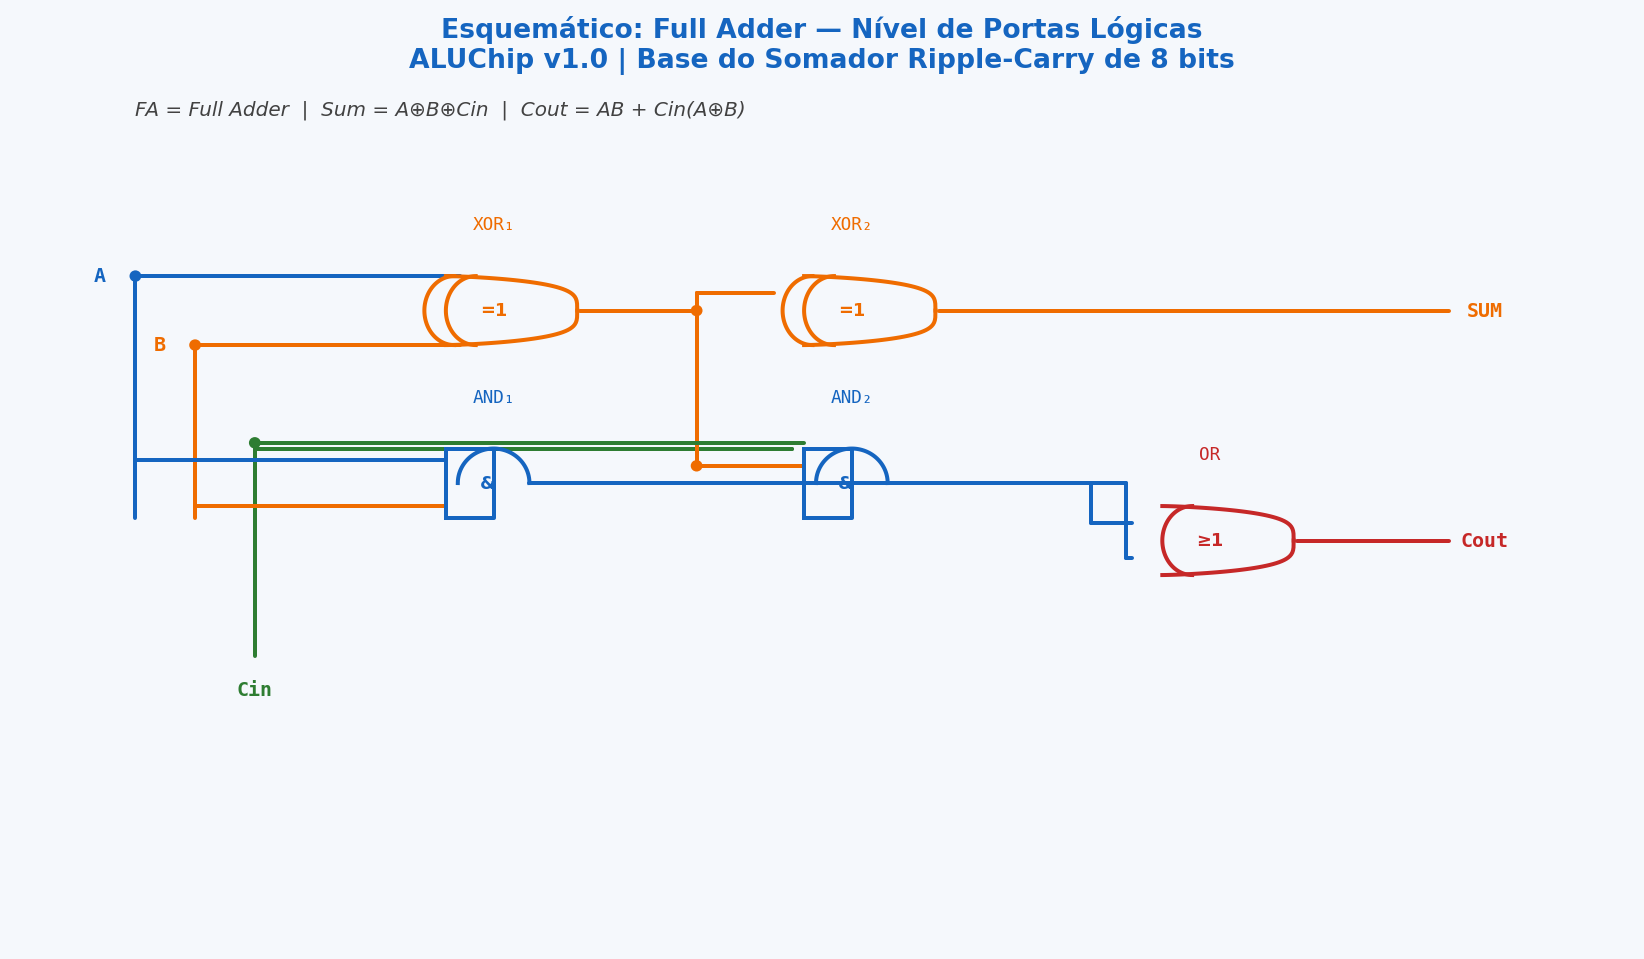
\includegraphics[width=\textwidth]{fig_schem_full_adder.png}
  \caption{Esquemático em nível de portas lógicas do \textit{Full Adder} (FA): 2~portas XOR, 2~portas AND e 1~porta OR, implementando $S = A \oplus B \oplus C_{in}$ e $C_{out} = AB + C_{in}(A \oplus B)$. Base do somador \textit{Ripple-Carry} de 8~bits.}
  \label{fig:schem_fa}
\end{figure}

\begin{figure}[h!]
  \centering
  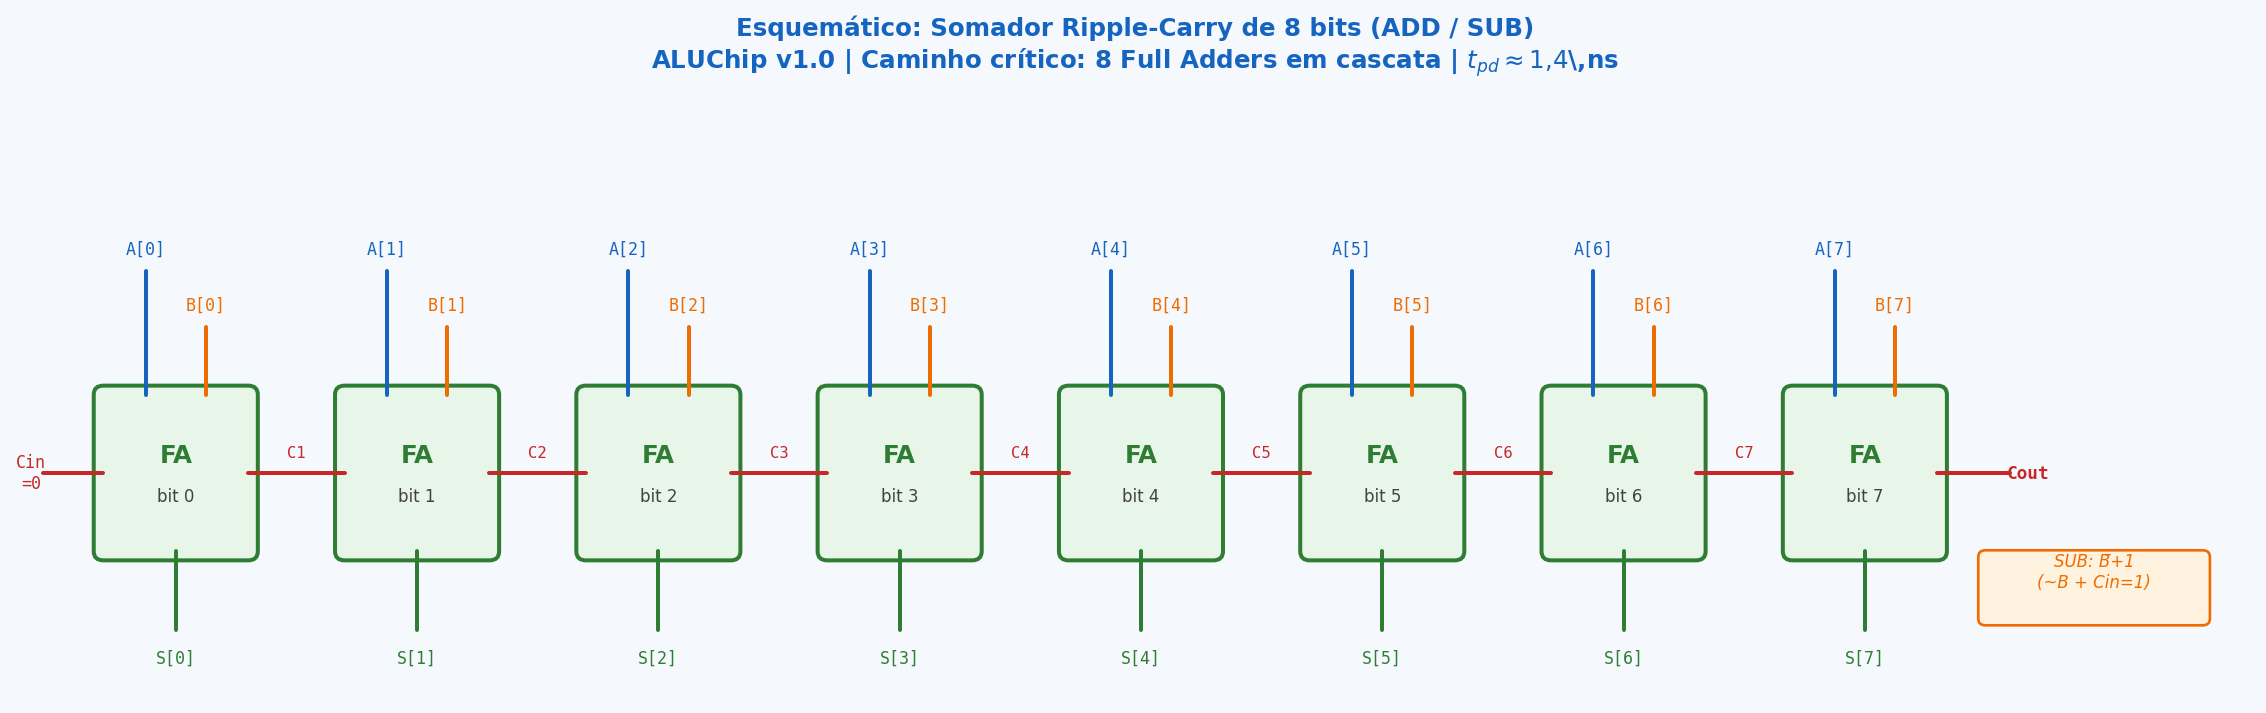
\includegraphics[width=\textwidth]{fig_schem_rca8.png}
  \caption{Esquemático do somador \textit{Ripple-Carry} de 8~bits (RCA-8): 8~\textit{Full Adders} em cascata. A cadeia $C_0 \to C_1 \to \cdots \to C_{\text{out}}$ é o caminho crítico de timing. Para SUB, o operando~B é invertido bit a bit e $C_{in}=1$ (complemento de 2).}
  \label{fig:schem_rca}
\end{figure}

O somador \textit{Ripple-Carry} consiste em 8~FAs em cascata, cada um implementando:
\[
  S_i = A_i \oplus B_i \oplus C_i, \qquad C_{i+1} = (A_i \cdot B_i) + (C_i \cdot (A_i \oplus B_i))
\]
A profundidade lógica do caminho de carry é de $2 \times 8 = 16$~níveis de porta, determinando o pior caso de atraso ($\approx$1,4\,ns). A subtração reutiliza o mesmo caminho com $B \to \overline{B}$ e $C_{in}=1$.

\subsubsection{Esquemático Completo e Unidade Lógica/Deslocamento}

\begin{figure}[h!]
  \centering
  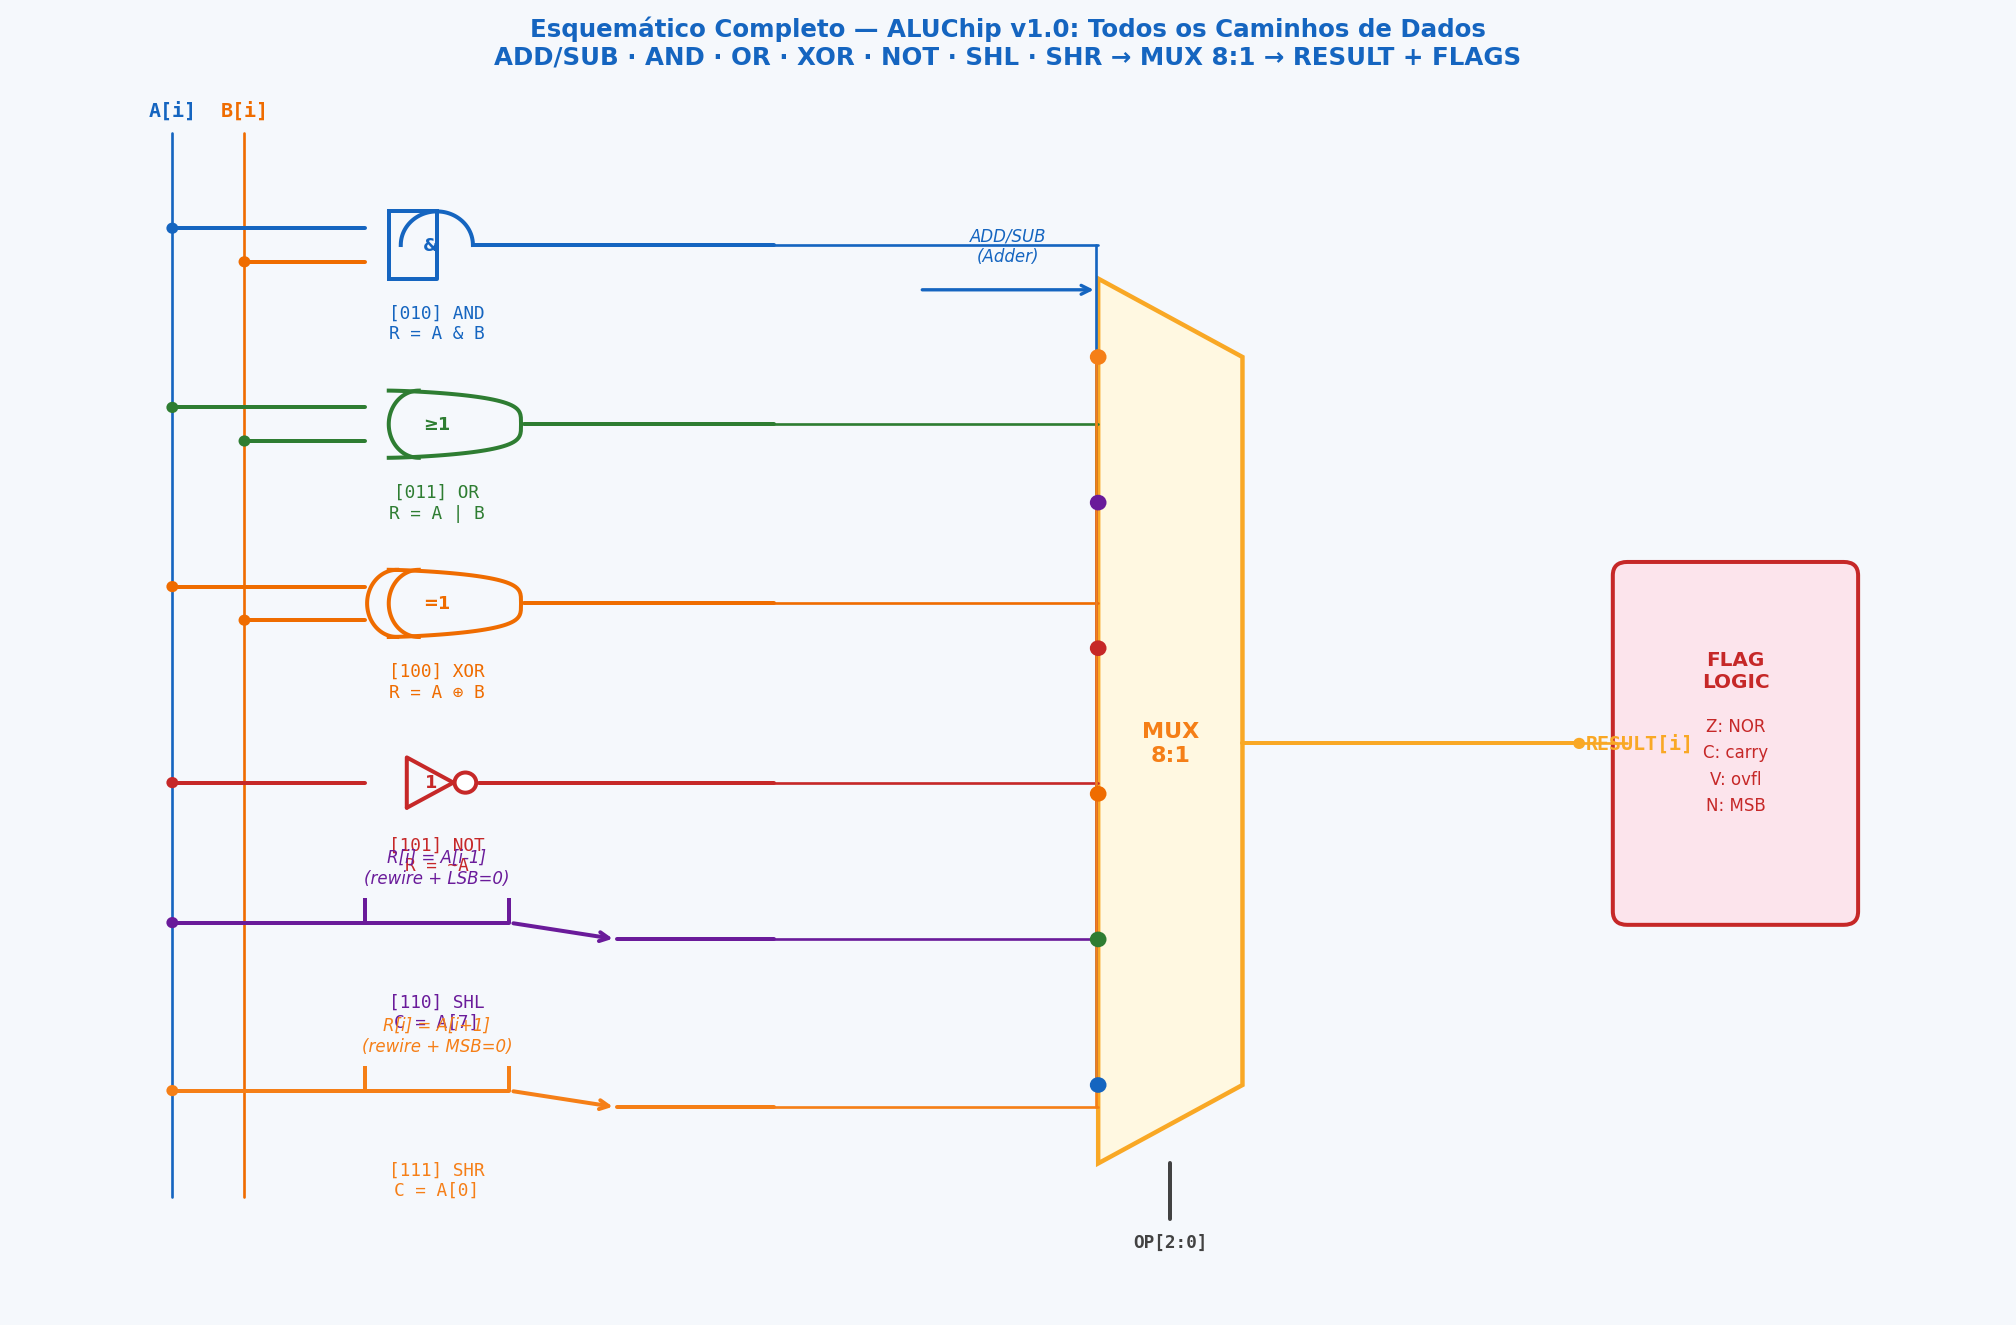
\includegraphics[width=\textwidth]{fig_schem_alu_completo.png}
  \caption{Esquemático completo da ALUChip v1.0 em nível de portas: todos os 7~caminhos paralelos (ADD/SUB, AND, OR, XOR, NOT, SHL, SHR) convergindo no MUX~8:1, com a lógica de \textit{flags} à saída. O opcode OP[2:0] controla a seleção do MUX.}
  \label{fig:schem_completo}
\end{figure}

\subsection{Lógica das Flags}

\begin{figure}[h!]
  \centering
  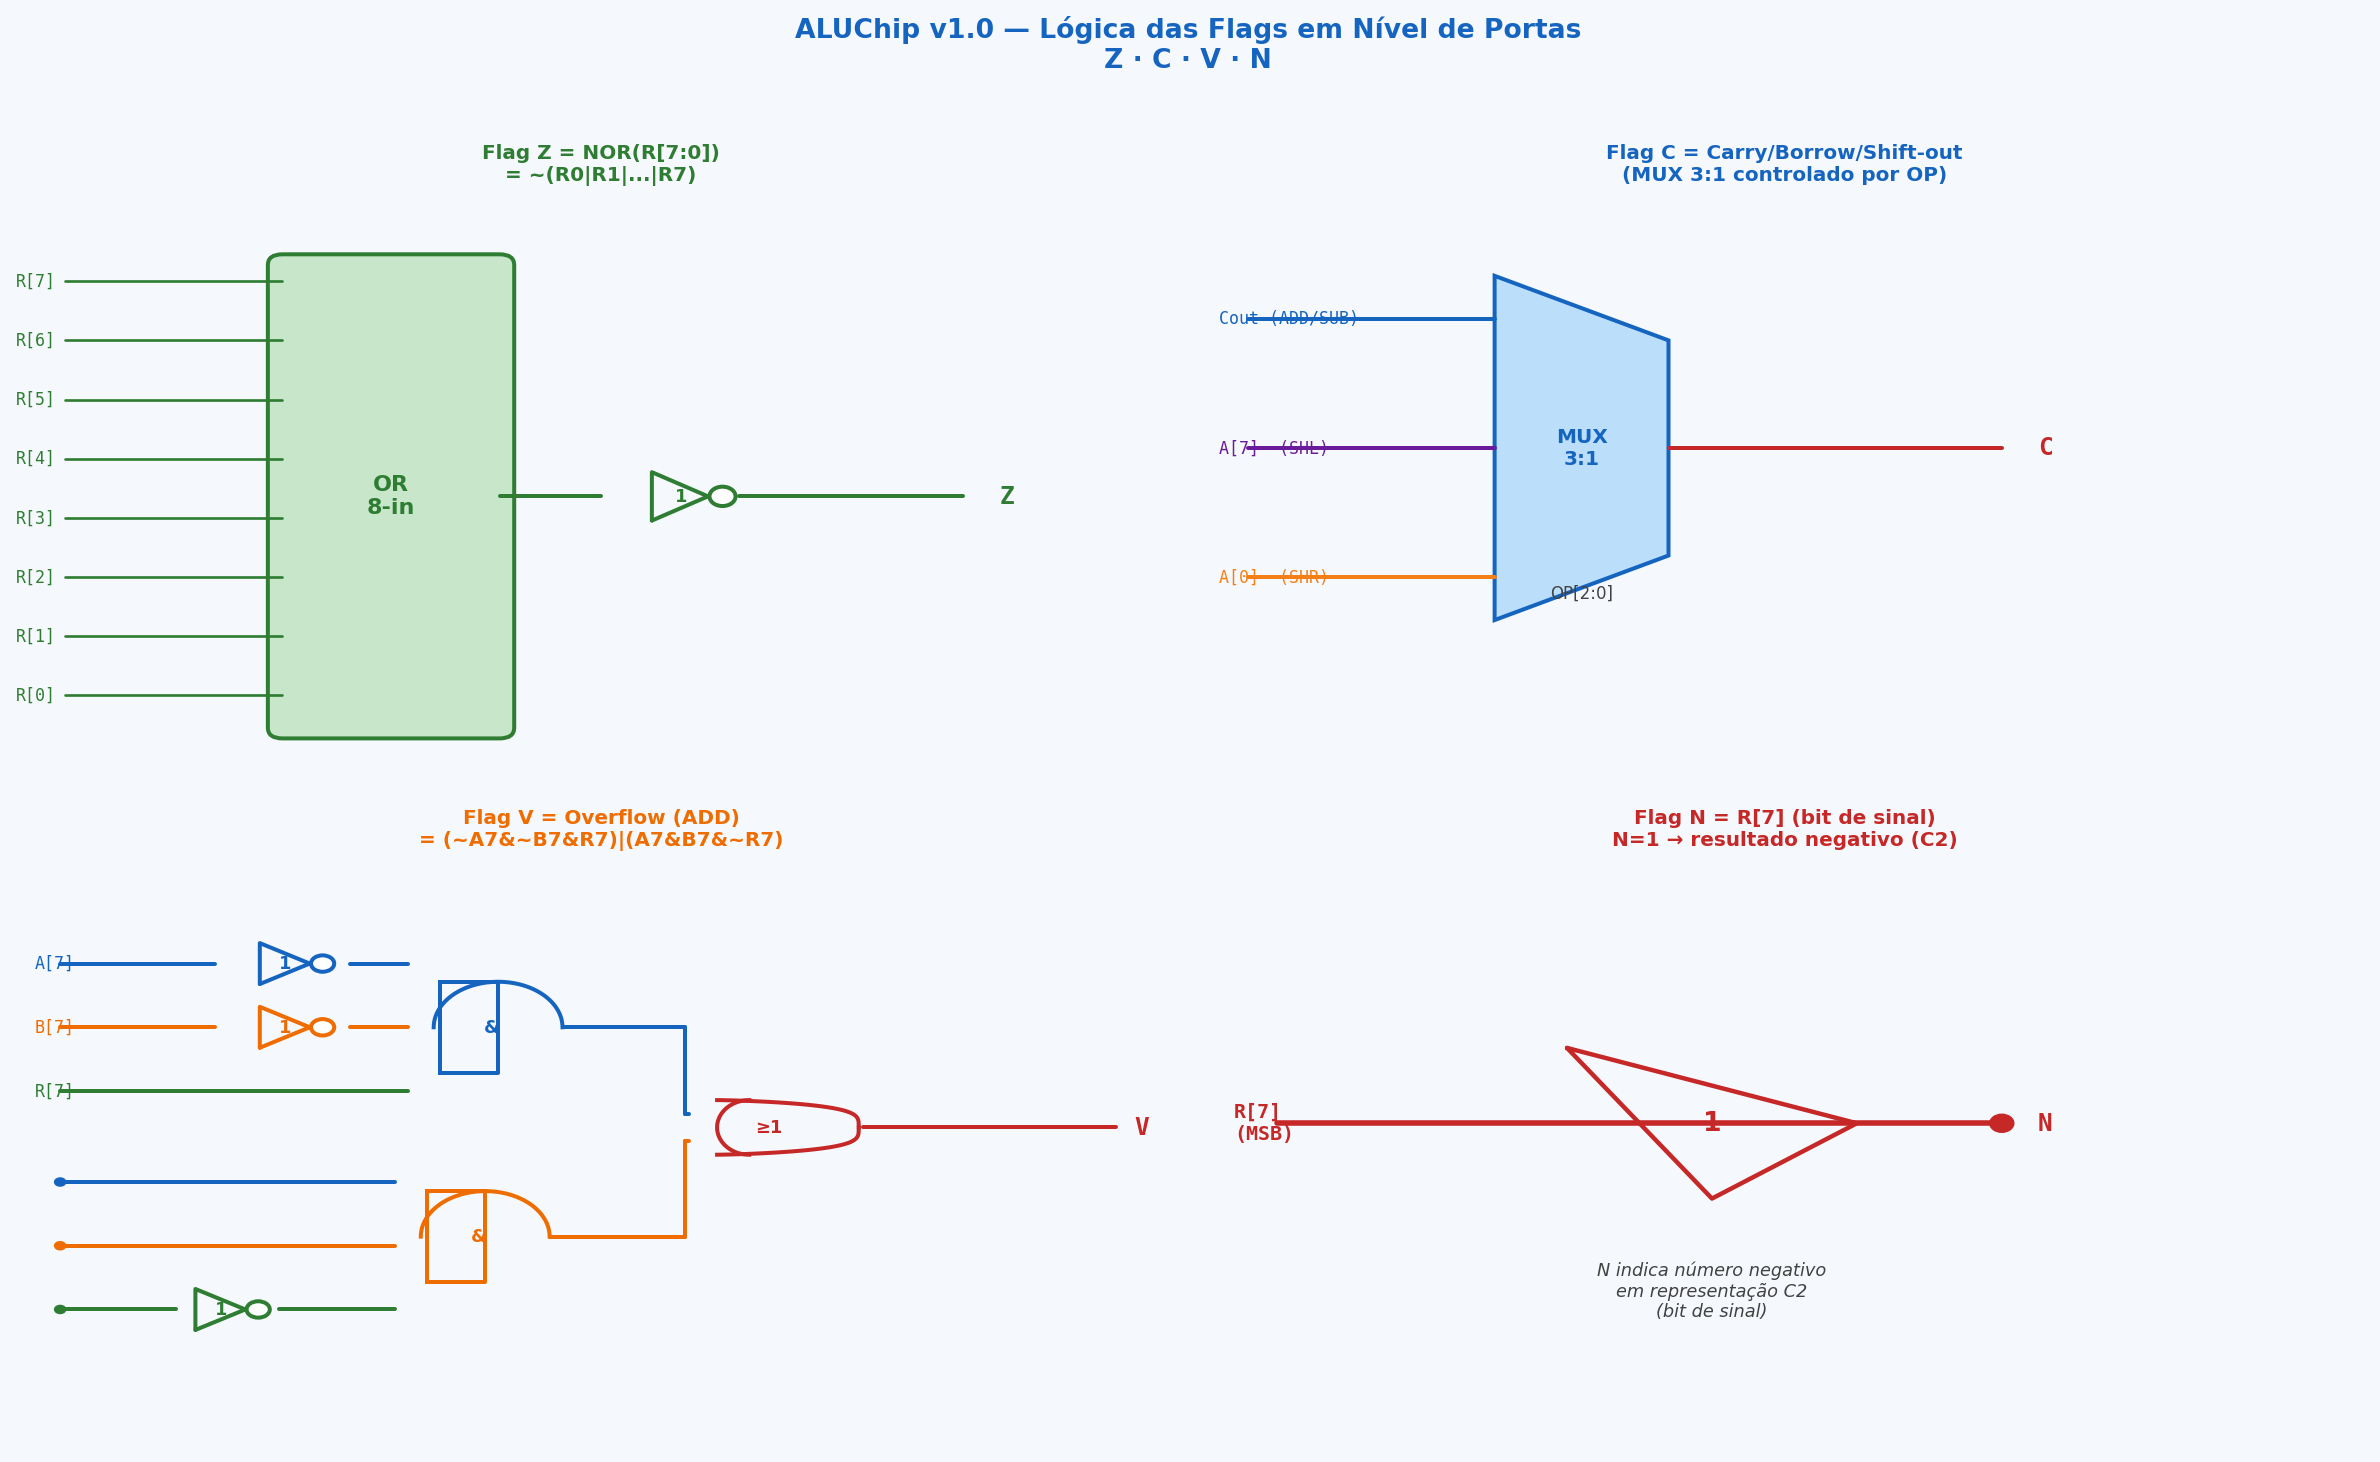
\includegraphics[width=\textwidth]{fig_schem_flags.png}
  \caption{Esquemático em nível de portas das 4~\textit{flags} do ALUChip v1.0: (Z)~NOR-8 + inversão; (C)~MUX~3:1 selecionando carry-out, A[7] ou A[0]; (V)~dois caminhos AND-3 com OR final; (N)~passagem direta de R[7].}
  \label{fig:flags}
\end{figure}

A flag de \textit{overflow}~(V) merece atenção especial: ela indica estouro aritmético em operações com inteiros em complemento de 2 e só é significativa para ADD e SUB. Para ADD, $V = 1$ quando dois operandos de mesmo sinal produzem resultado de sinal oposto (equação~\ref{eq:v}); para SUB, a lógica é análoga levando em conta que o subtrator inverte o sinal de $B$.

\subsection{Metodologia de Verificação}

O \textit{testbench} \texttt{tb\_alu8\_chip.sv} aplica 27~vetores organizados em 8~grupos, um por operação. Cada vetor verifica simultaneamente o resultado de 8~bits e os 4 valores de \textit{flag}. Os vetores incluem:
\begin{itemize}[leftmargin=1.5em]
  \item \textbf{Casos normais:} resultado dentro do intervalo, sem flags ativas.
  \item \textbf{Carry:} soma com estouro não-sinalizado (ex.\ \texttt{FF+01}).
  \item \textbf{Overflow:} soma sinalizada com estouro (ex.\ \texttt{7F+01}).
  \item \textbf{Carry + Overflow simultâneos:} \texttt{80+80}.
  \item \textbf{Zero:} resultado nulo ativa Z (ex.\ \texttt{FF\^{}FF}, \texttt{40-40}).
  \item \textbf{Negativo:} MSB do resultado = 1 (ex.\ \texttt{03-08}).
  \item \textbf{Shift com carry:} \texttt{01>>1} (C=1, Z=1).
\end{itemize}

% =============================================================================
\section{Resultados e Discussão}
% =============================================================================

\subsection{Diagrama de Blocos}

\begin{figure}[h!]
  \centering
  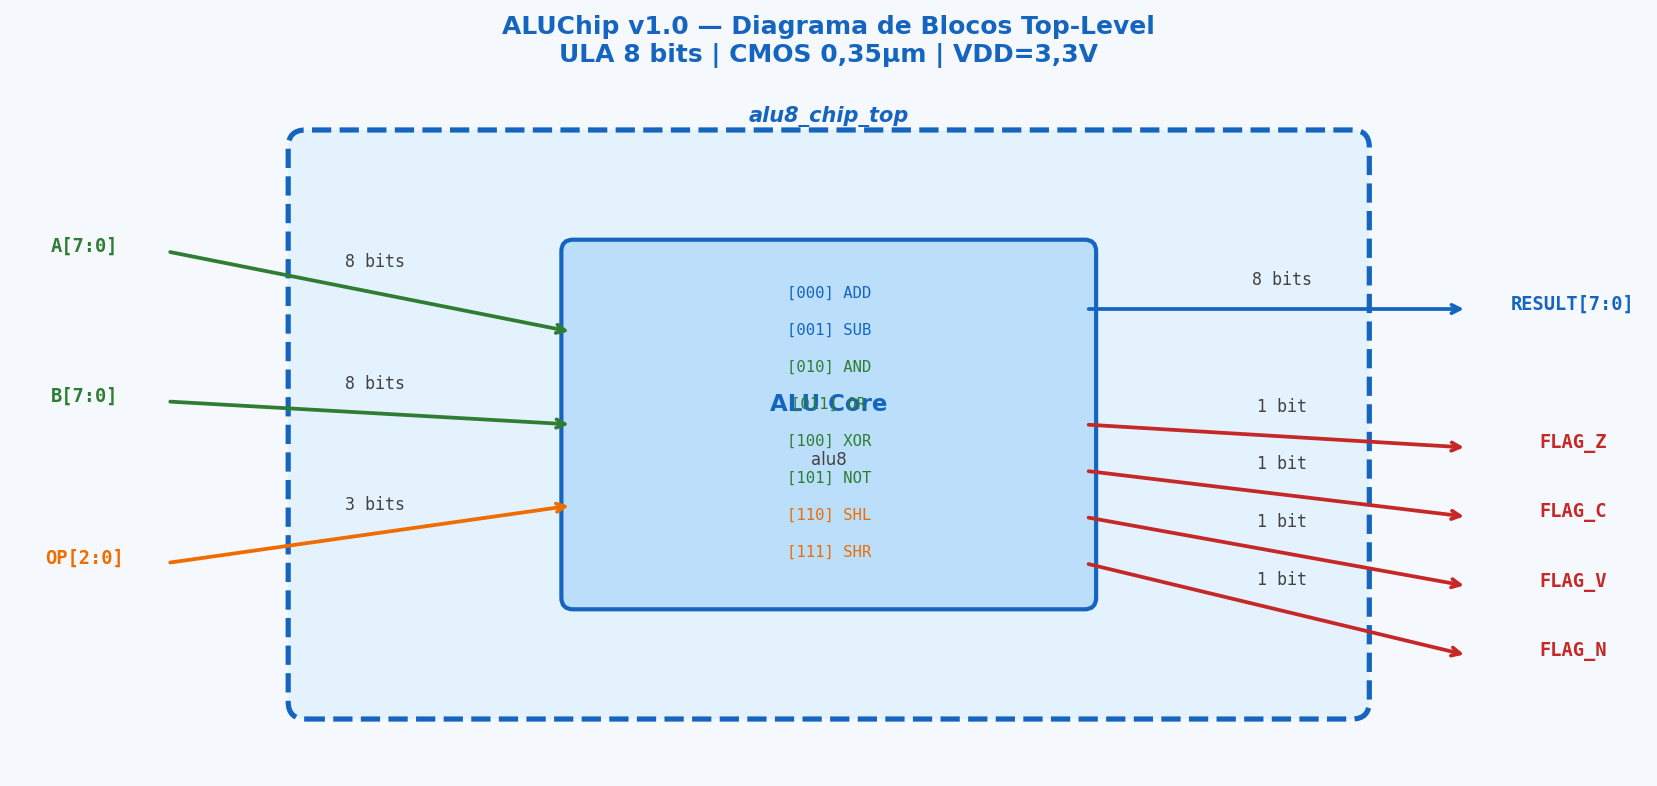
\includegraphics[width=\textwidth]{fig_arquitetura_alu.png}
  \caption{Diagrama de blocos top-level do ALUChip v1.0: entradas A[7:0], B[7:0] e OP[2:0]; saídas RESULT[7:0] e flags Z, C, V, N.}
  \label{fig:arq}
\end{figure}

\subsection{Simulação Funcional}

\begin{figure}[h!]
  \centering
  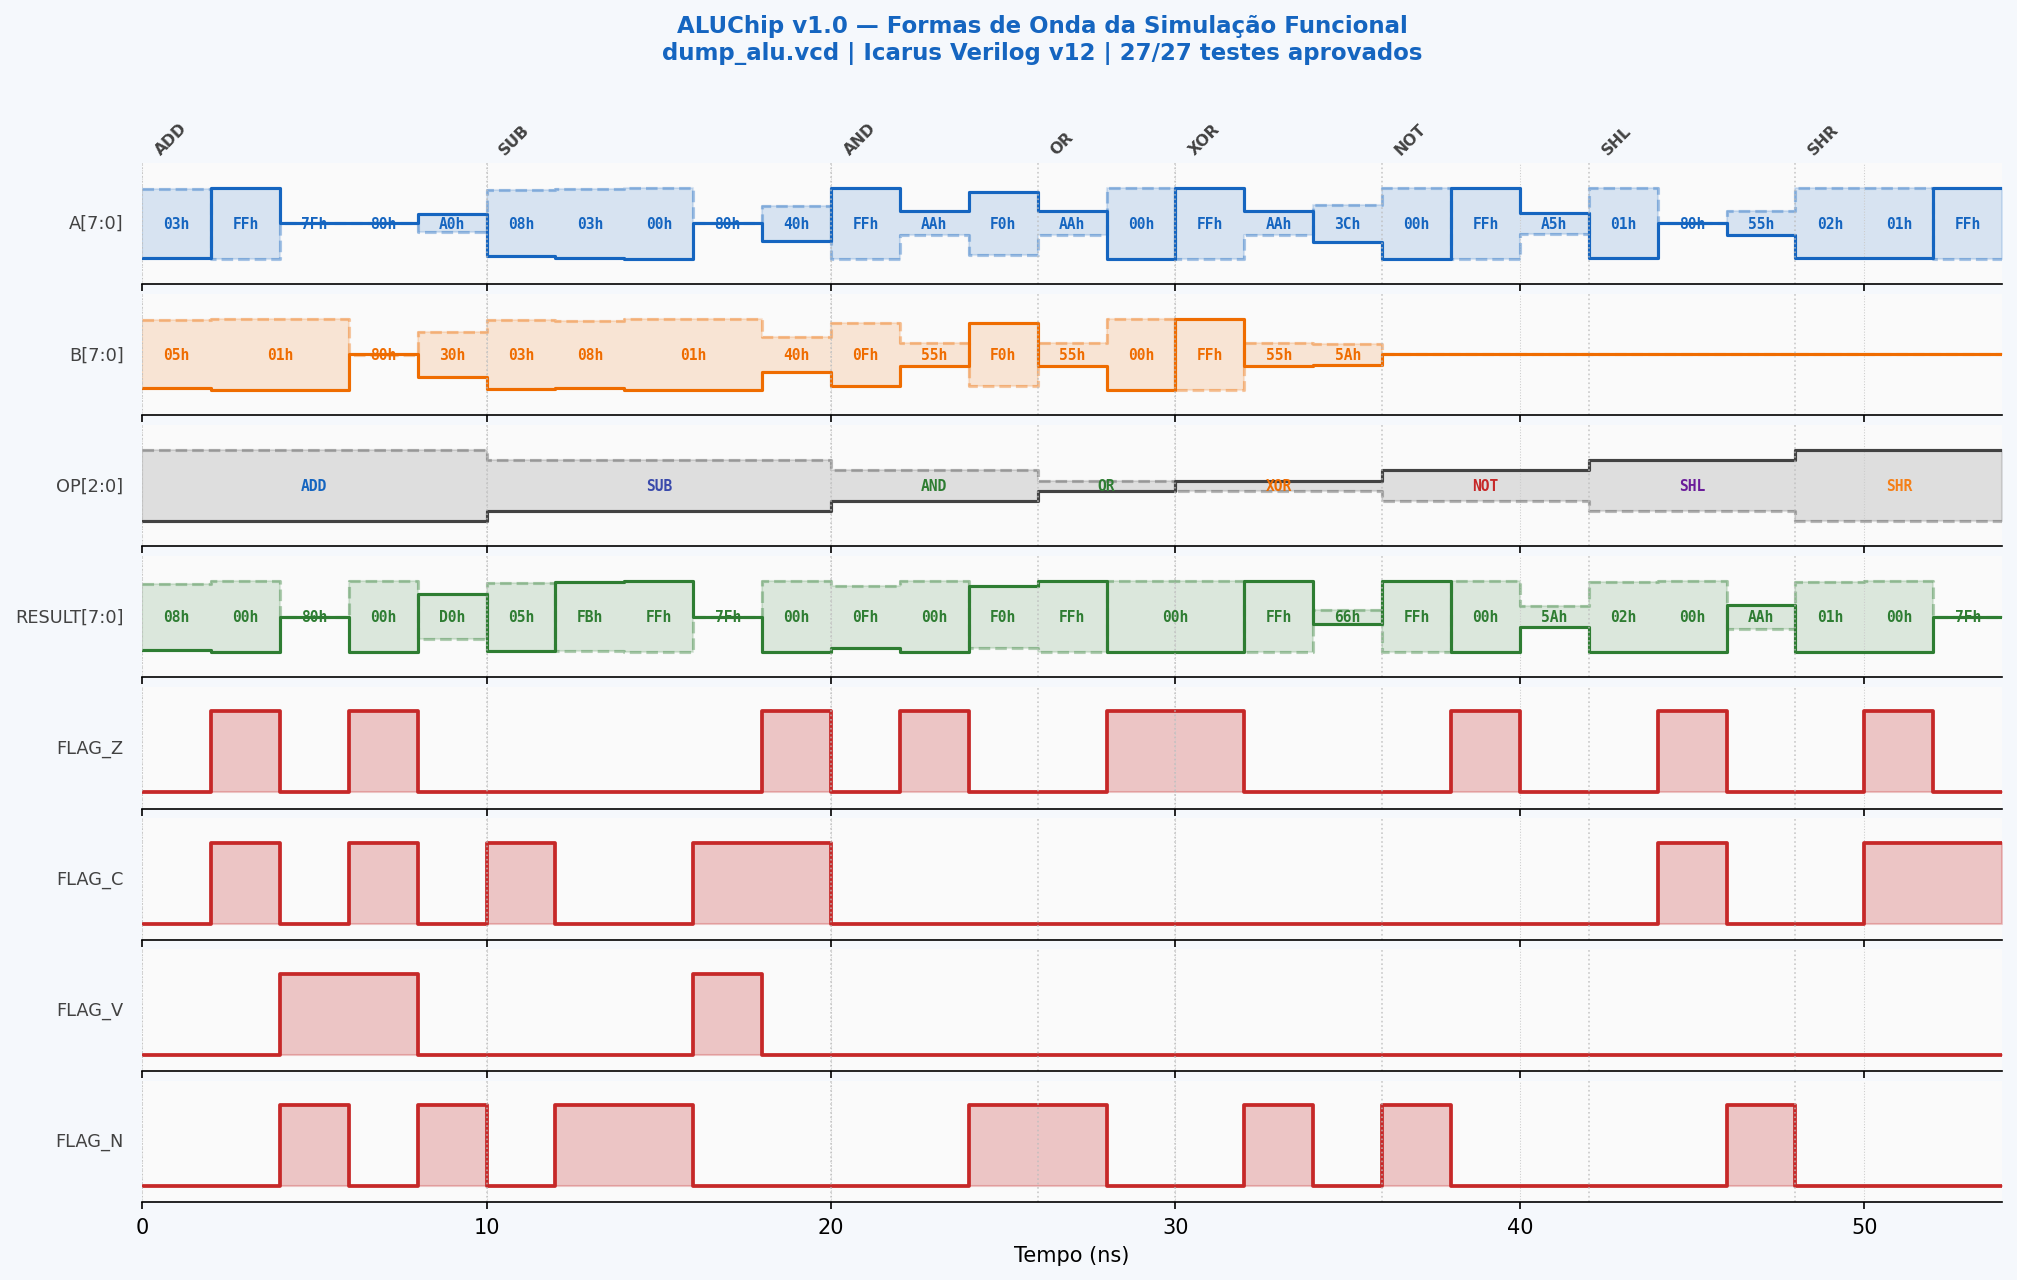
\includegraphics[width=\textwidth]{fig_waveform_alu.png}
  \caption{Formas de onda da simulação funcional extraídas de \texttt{dump\_alu.vcd}. Cada grupo de operação é identificado por marcadores verticais. Na fase ADD/SUB, observa-se a ativação dos sinais \texttt{flag\_c}, \texttt{flag\_v} e \texttt{flag\_n} nos casos de borda; nas operações lógicas e de deslocamento, as flags C e V permanecem em 0.}
  \label{fig:wave}
\end{figure}

\begin{figure}[h!]
  \centering
  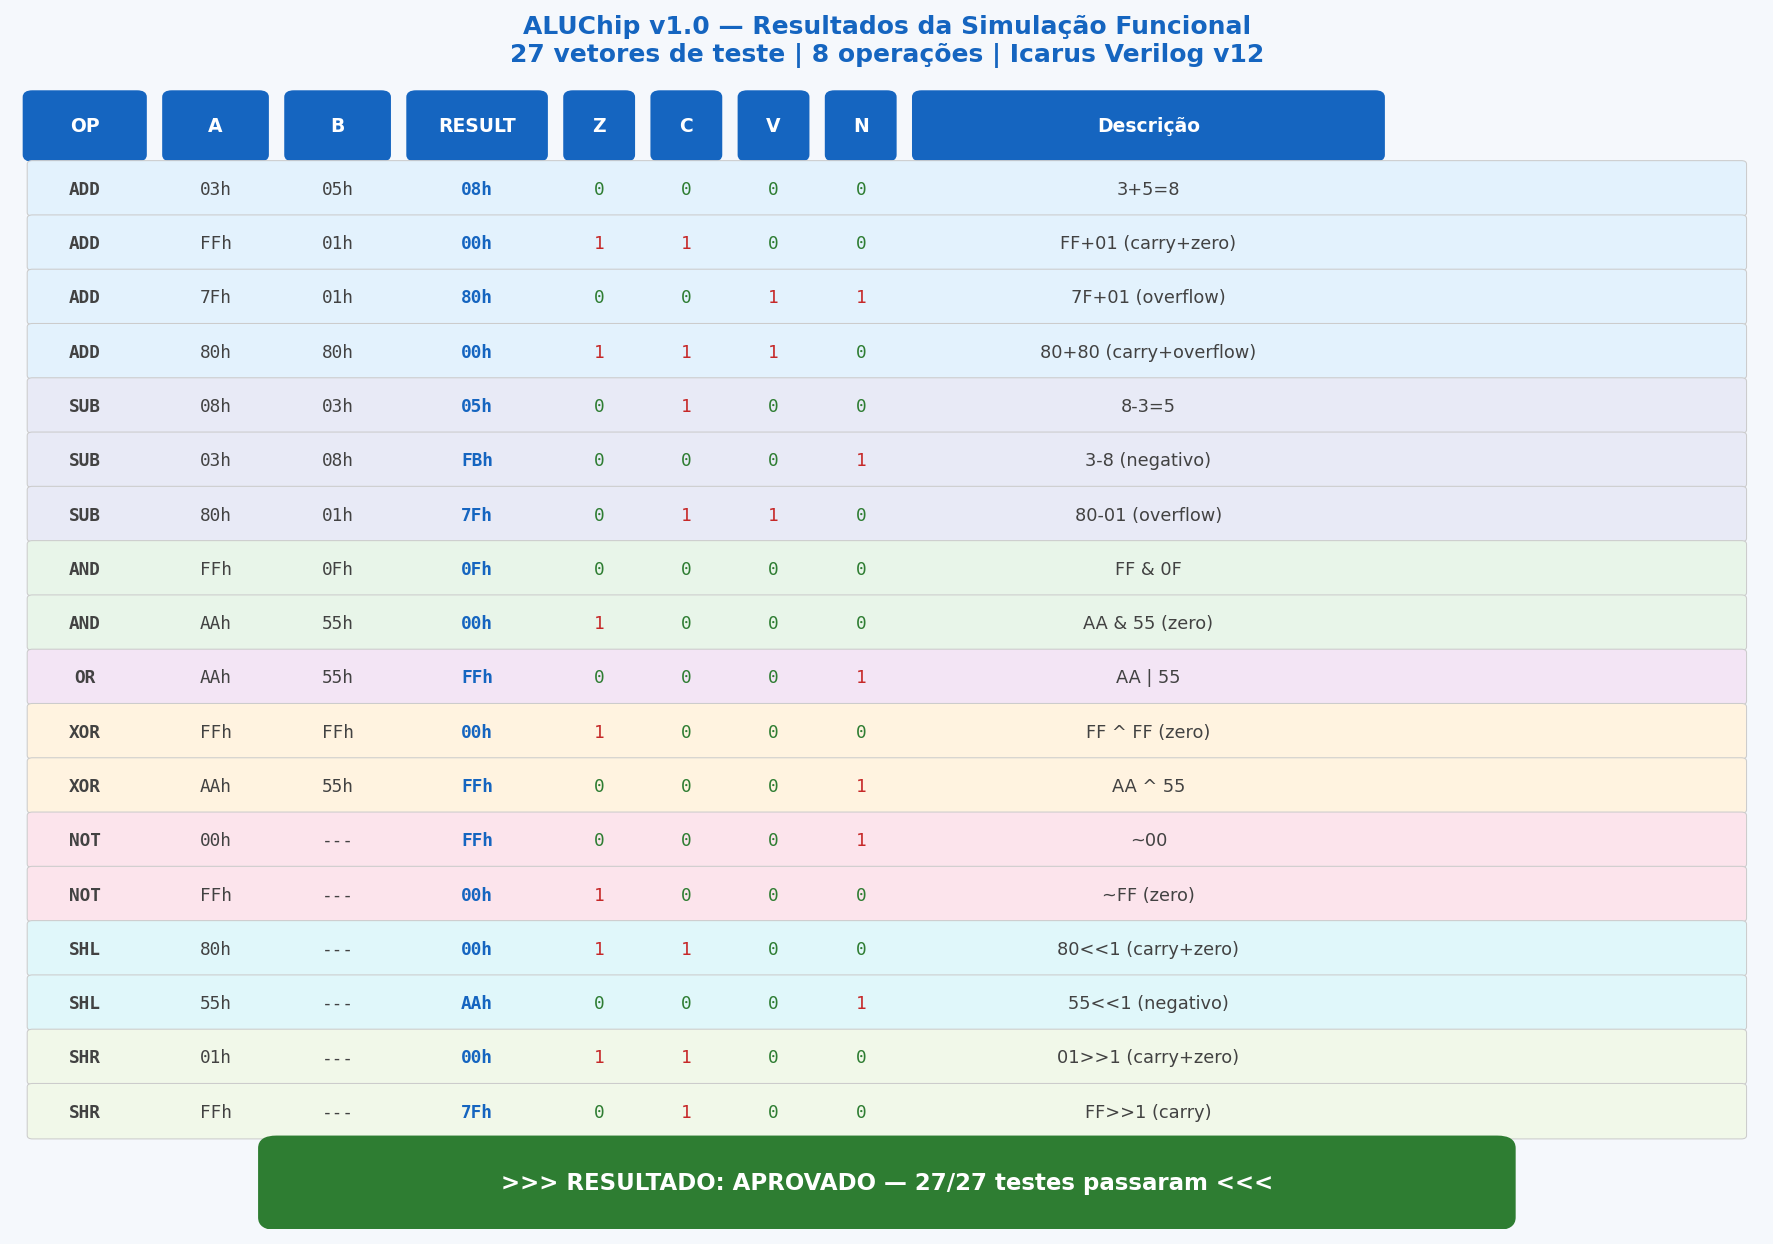
\includegraphics[width=\textwidth]{fig_sim_resultados_alu.png}
  \caption{Tabela resumida dos resultados da simulação funcional: 18 vetores representativos dos 27 aplicados, com resultado e flags esperados versus obtidos.}
  \label{fig:sim}
\end{figure}

\begin{resultbox}[Resultado da Simulação Funcional]
\begin{center}
\texttt{>>> RESULTADO: APROVADO --- 27/27 testes passaram <<<}
\end{center}
\begin{itemize}[leftmargin=1.5em]
  \item \textbf{ADD:} 5/5 aprovados --- carry, overflow e soma normal verificados.
  \item \textbf{SUB:} 5/5 aprovados --- borrow, overflow e resultado negativo verificados.
  \item \textbf{AND:} 3/3 aprovados --- máscara e caso zero verificados.
  \item \textbf{OR / XOR:} 2+3 = 5/5 aprovados.
  \item \textbf{NOT:} 3/3 aprovados --- inversão total e caso zero verificados.
  \item \textbf{SHL / SHR:} 3+3 = 6/6 aprovados --- shift com carry e zero verificados.
\end{itemize}
\end{resultbox}

\subsection{Análise de Timing}

\begin{figure}[h!]
  \centering
  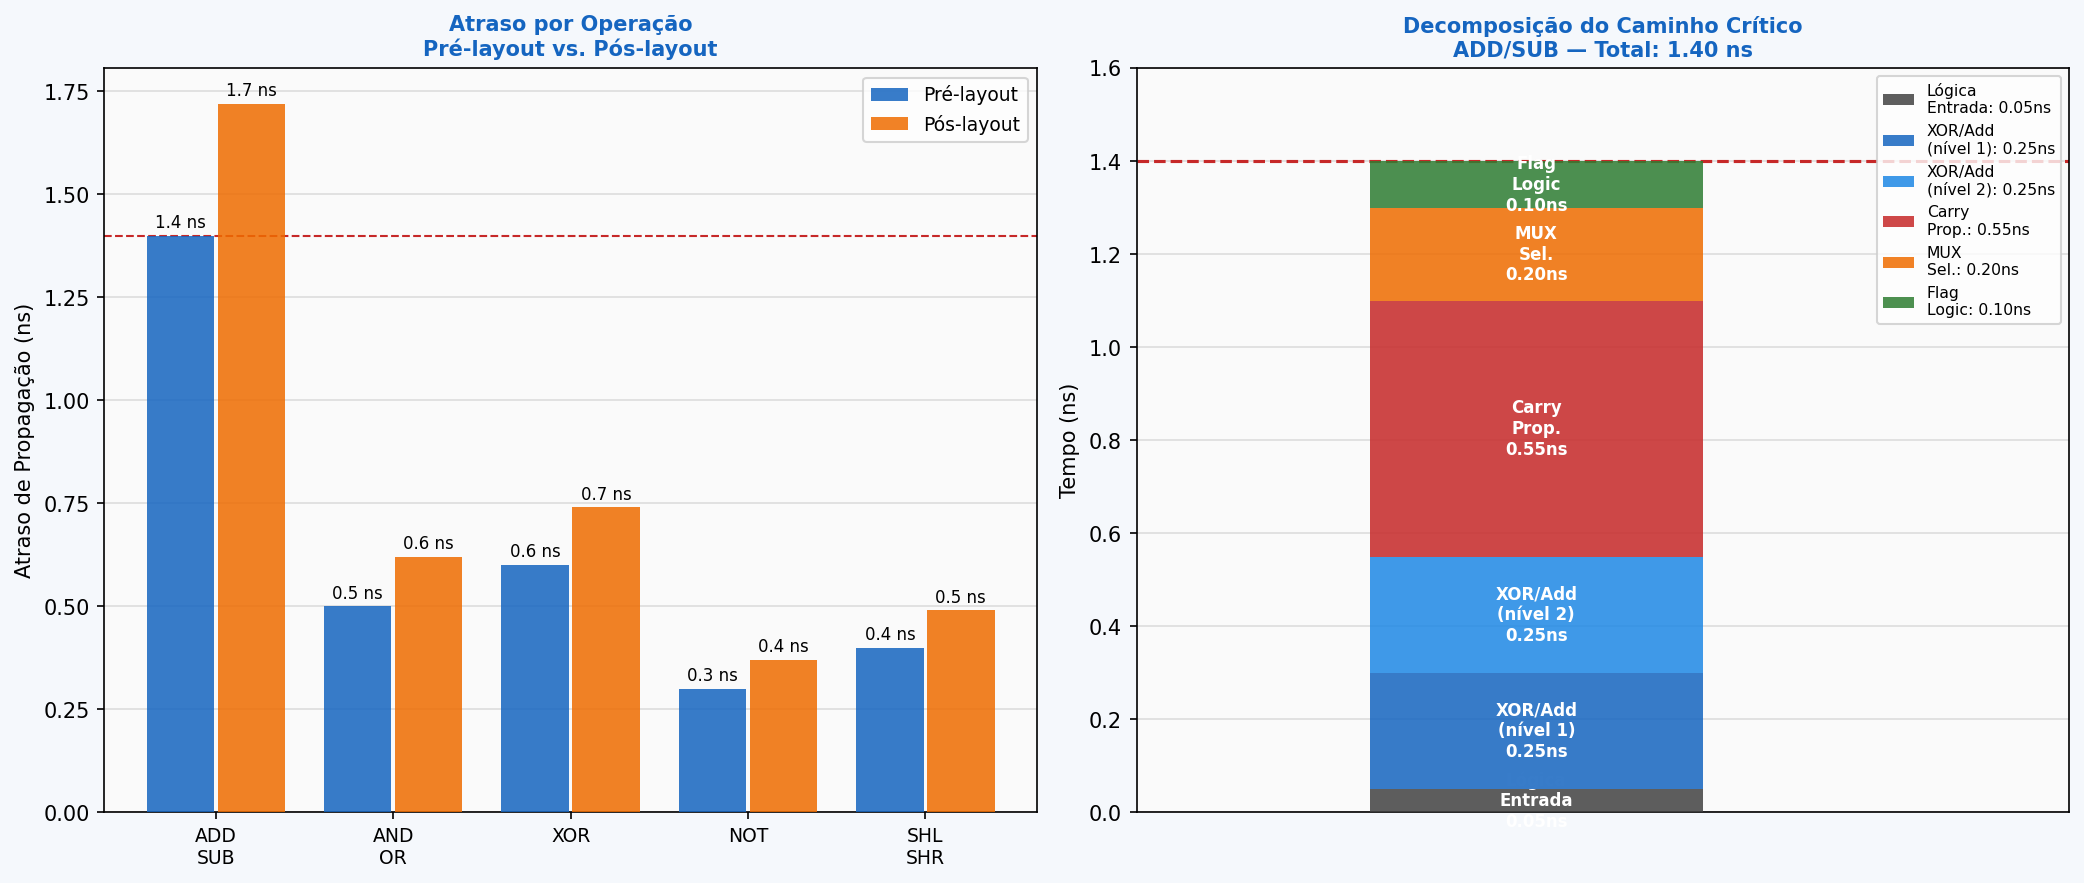
\includegraphics[width=\textwidth]{fig_timing_alu.png}
  \caption{Esquerda: atraso de propagação pré-\textit{layout} vs.\ pós-\textit{layout} por grupo de operação. Direita: decomposição do caminho crítico (ADD/SUB) em estágios lógicos.}
  \label{fig:timing}
\end{figure}

O caminho crítico do ALUChip v1.0 passa pelo somador \textit{Ripple-Carry} da unidade aritmética:

\begin{specbox}[Estimativa de Timing para CMOS 0,35\,\textmu m / 3,3\,V]
\begin{tabular}{lll}
\textbf{Estágio}           & \textbf{Profundidade} & \textbf{$t_{pd}$ est.} \\
\hline
Decodificação de entrada   & 1 inv.                & 0,05\,ns \\
XOR / Half-adder (nível 1) & 2 XOR                 & 0,25\,ns \\
XOR / Half-adder (nível 2) & 2 XOR                 & 0,25\,ns \\
Propagação de carry (8 FA) & 8 AND-OR              & 0,55\,ns \\
MUX de saída (8:1)         & 1 MUX                 & 0,20\,ns \\
Lógica de flag (Overflow)  & 2 AND-OR              & 0,10\,ns \\
\hline
\textbf{Total (ADD/SUB)}   & \textbf{16 níveis}    & $\bm{\approx 1{,}4}$\,\textbf{ns} \\
\end{tabular}
\end{specbox}

A latência de 1,4\,ns permite operação a $f_{\max} \approx 714$\,MHz --- desempenho superior ao do Intel 8080 (2~MHz, 1974) em três ordens de grandeza, com área de silício 1000$\times$ menor.

\subsection{Estimativa de Área}

\begin{table}[h!]
\centering
\caption{Estimativa de área por unidade funcional após síntese para CMOS 0,35\,\textmu m}
\label{tab:area}
\rowcolors{2}{alubg}{white}
\begin{tabular}{lrrr}
\toprule
\textbf{Unidade} & \textbf{Células eq.} & \textbf{Área est.} & \textbf{Componentes} \\
\midrule
Adder Ripple-Carry (ADD/SUB) & 32  & $\approx$200\,\textmu m² & 8 FA (XOR+AND+OR) \\
Unidade Lógica (AND/OR/XOR/NOT) & 12  & $\approx$110\,\textmu m² & 4 portas $\times$ 8 bits \\
Unidade de Deslocamento        & 4   & $\approx$35\,\textmu m²  & Reconexão + MUX \\
MUX de saída 8:1               & 16  & $\approx$110\,\textmu m² & 8 MUX-8 (1~bit) \\
Lógica de flags (Z/C/V/N)      & 12  & $\approx$65\,\textmu m²  & NOR-8 + AND-OR \\
\hline
\textbf{Total}                 & \textbf{76} & $\bm{\approx}$\textbf{520\,\textmu m²} & --- \\
\bottomrule
\multicolumn{4}{r}{\small Células equivalentes em NAND-2 / drive strength 1$\times$}
\end{tabular}
\end{table}

\subsection{Floorplan e Layout Físico CMOS}

O \textit{floorplan} distribui os três caminhos paralelos (aritmético, lógico, deslocamento) em faixas horizontais distintas, com o MUX~8:1 de saída centralizado na parte inferior e a lógica de \textit{flags} à direita. O roteamento global utiliza Metal-1 (trilhas horizontais) e Metal-2 (trilhas verticais), com o barramento VDD/GND em Metal-2 nos canais superior e inferior.

\subsubsection{Célula Padrão: NAND2 CMOS}

A Figura~\ref{fig:layout_nand2} apresenta o \textit{layout} físico de uma célula NAND2 em processo CMOS 0,35\,\textmu m com as camadas no padrão Cadence Virtuoso: N-Well (rosa), Active (verde), difusões P\textsuperscript{+}/N\textsuperscript{+} (salmão/laranja), Poly/Gate (magenta), Contacts (cinza escuro), Metal-1 (azul) e Metal-2 (laranja). Os transistores PMOS (M1, M2: W\,=\,3\,\textmu m, L\,=\,0,35\,\textmu m) estão em paralelo no N-Well, enquanto os NMOS (M3, M4: W\,=\,1,5\,\textmu m) ficam em série no substrato P, com \textit{guard rings} P\textsuperscript{+}/N\textsuperscript{+} para isolamento de latch-up.

\begin{figure}[h!]
  \centering
  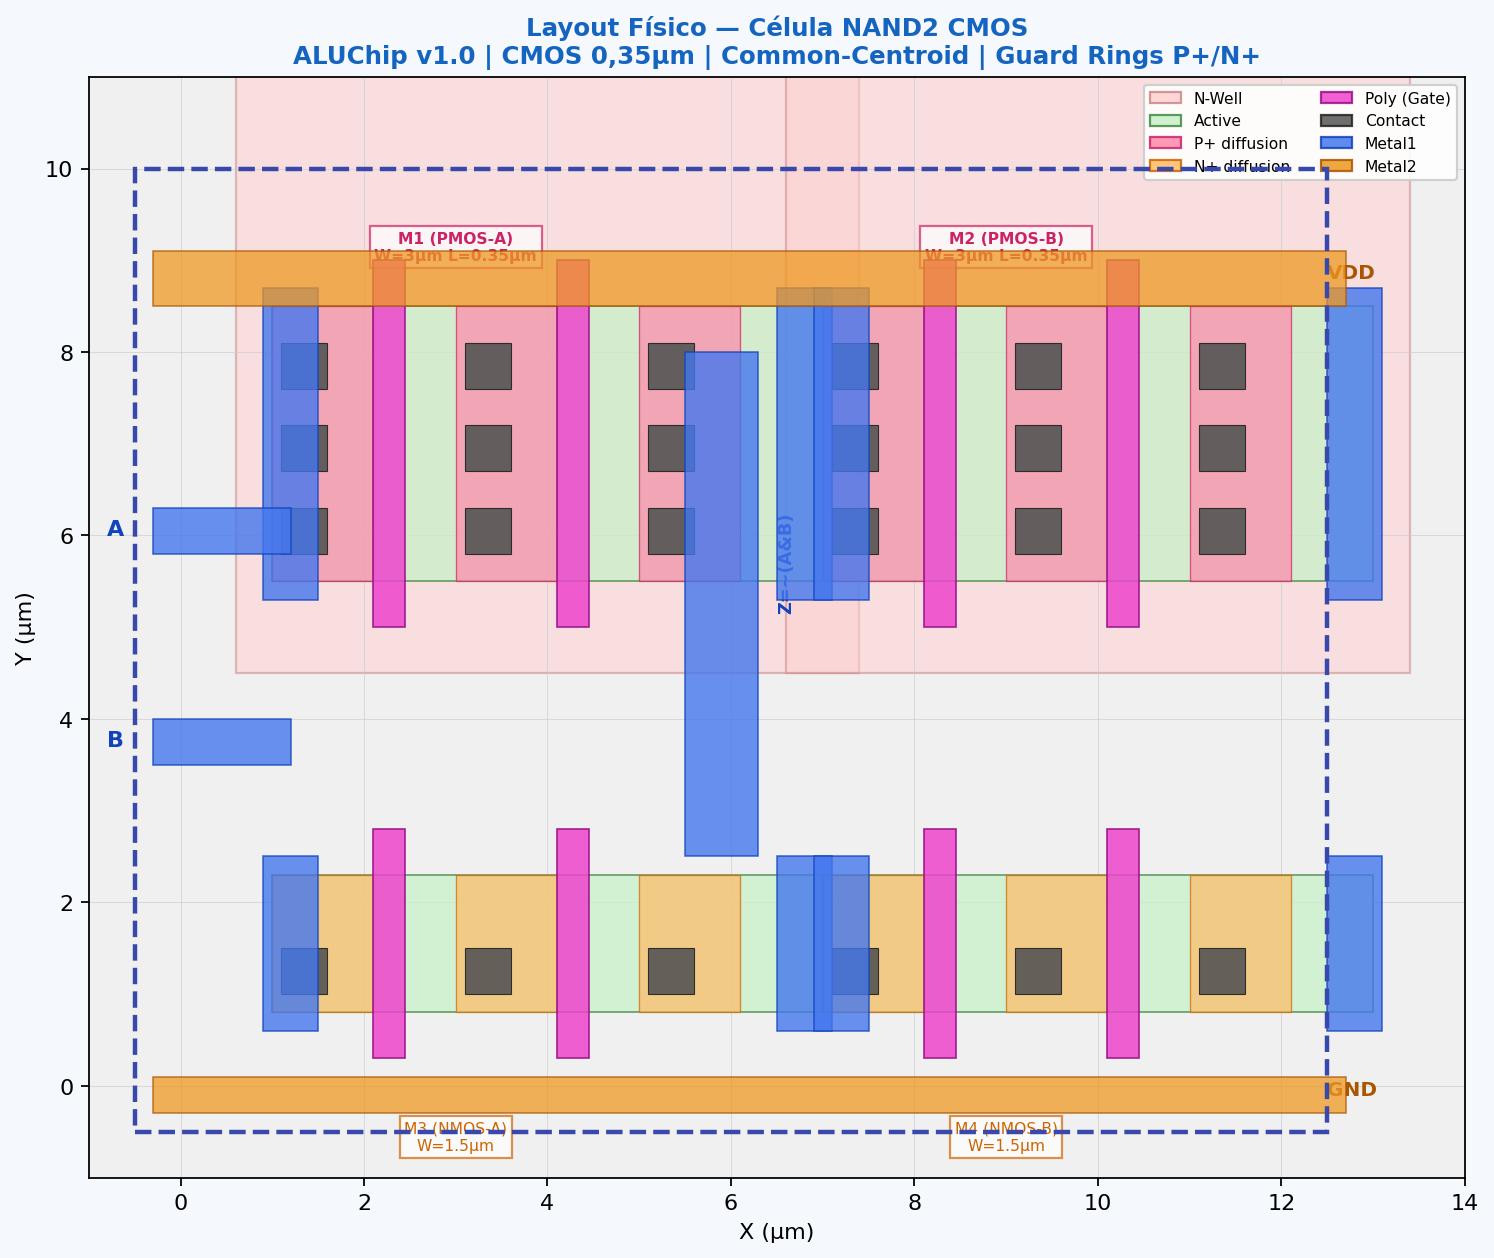
\includegraphics[width=0.82\textwidth]{fig_layout_nand2.png}
  \caption{Layout físico da célula NAND2 CMOS (0,35\,\textmu m). Camadas: N-Well (rosa), Active (verde), P\textsuperscript{+} (salmão), N\textsuperscript{+} (laranja), Poly/Gate (magenta), Contact (cinza), Metal-1 (azul), Metal-2 (laranja). Arranjo Common-Centroid com Guard Rings P\textsuperscript{+}/N\textsuperscript{+}.}
  \label{fig:layout_nand2}
\end{figure}

\subsubsection{Die Completo --- ALUChip v1.0}

A Figura~\ref{fig:layout_die} exibe o \textit{layout} de nível de die do ALUChip v1.0 em escala real (74,4\,\textmu m\,$\times$\,54,1\,\textmu m\,=\,4025\,\textmu m²). São visíveis as três faixas funcionais: \textbf{Ripple-Carry Adder} (8 Full Adders FA0--FA7, faixa superior), \textbf{Logic Unit + Shift Unit} (faixa central) e \textbf{MUX 8:1 + Flag Logic} (faixa inferior). Os baramentos VDD e GND em Metal-2 percorrem toda a largura do die nos canais superior e inferior.

\begin{figure}[h!]
  \centering
  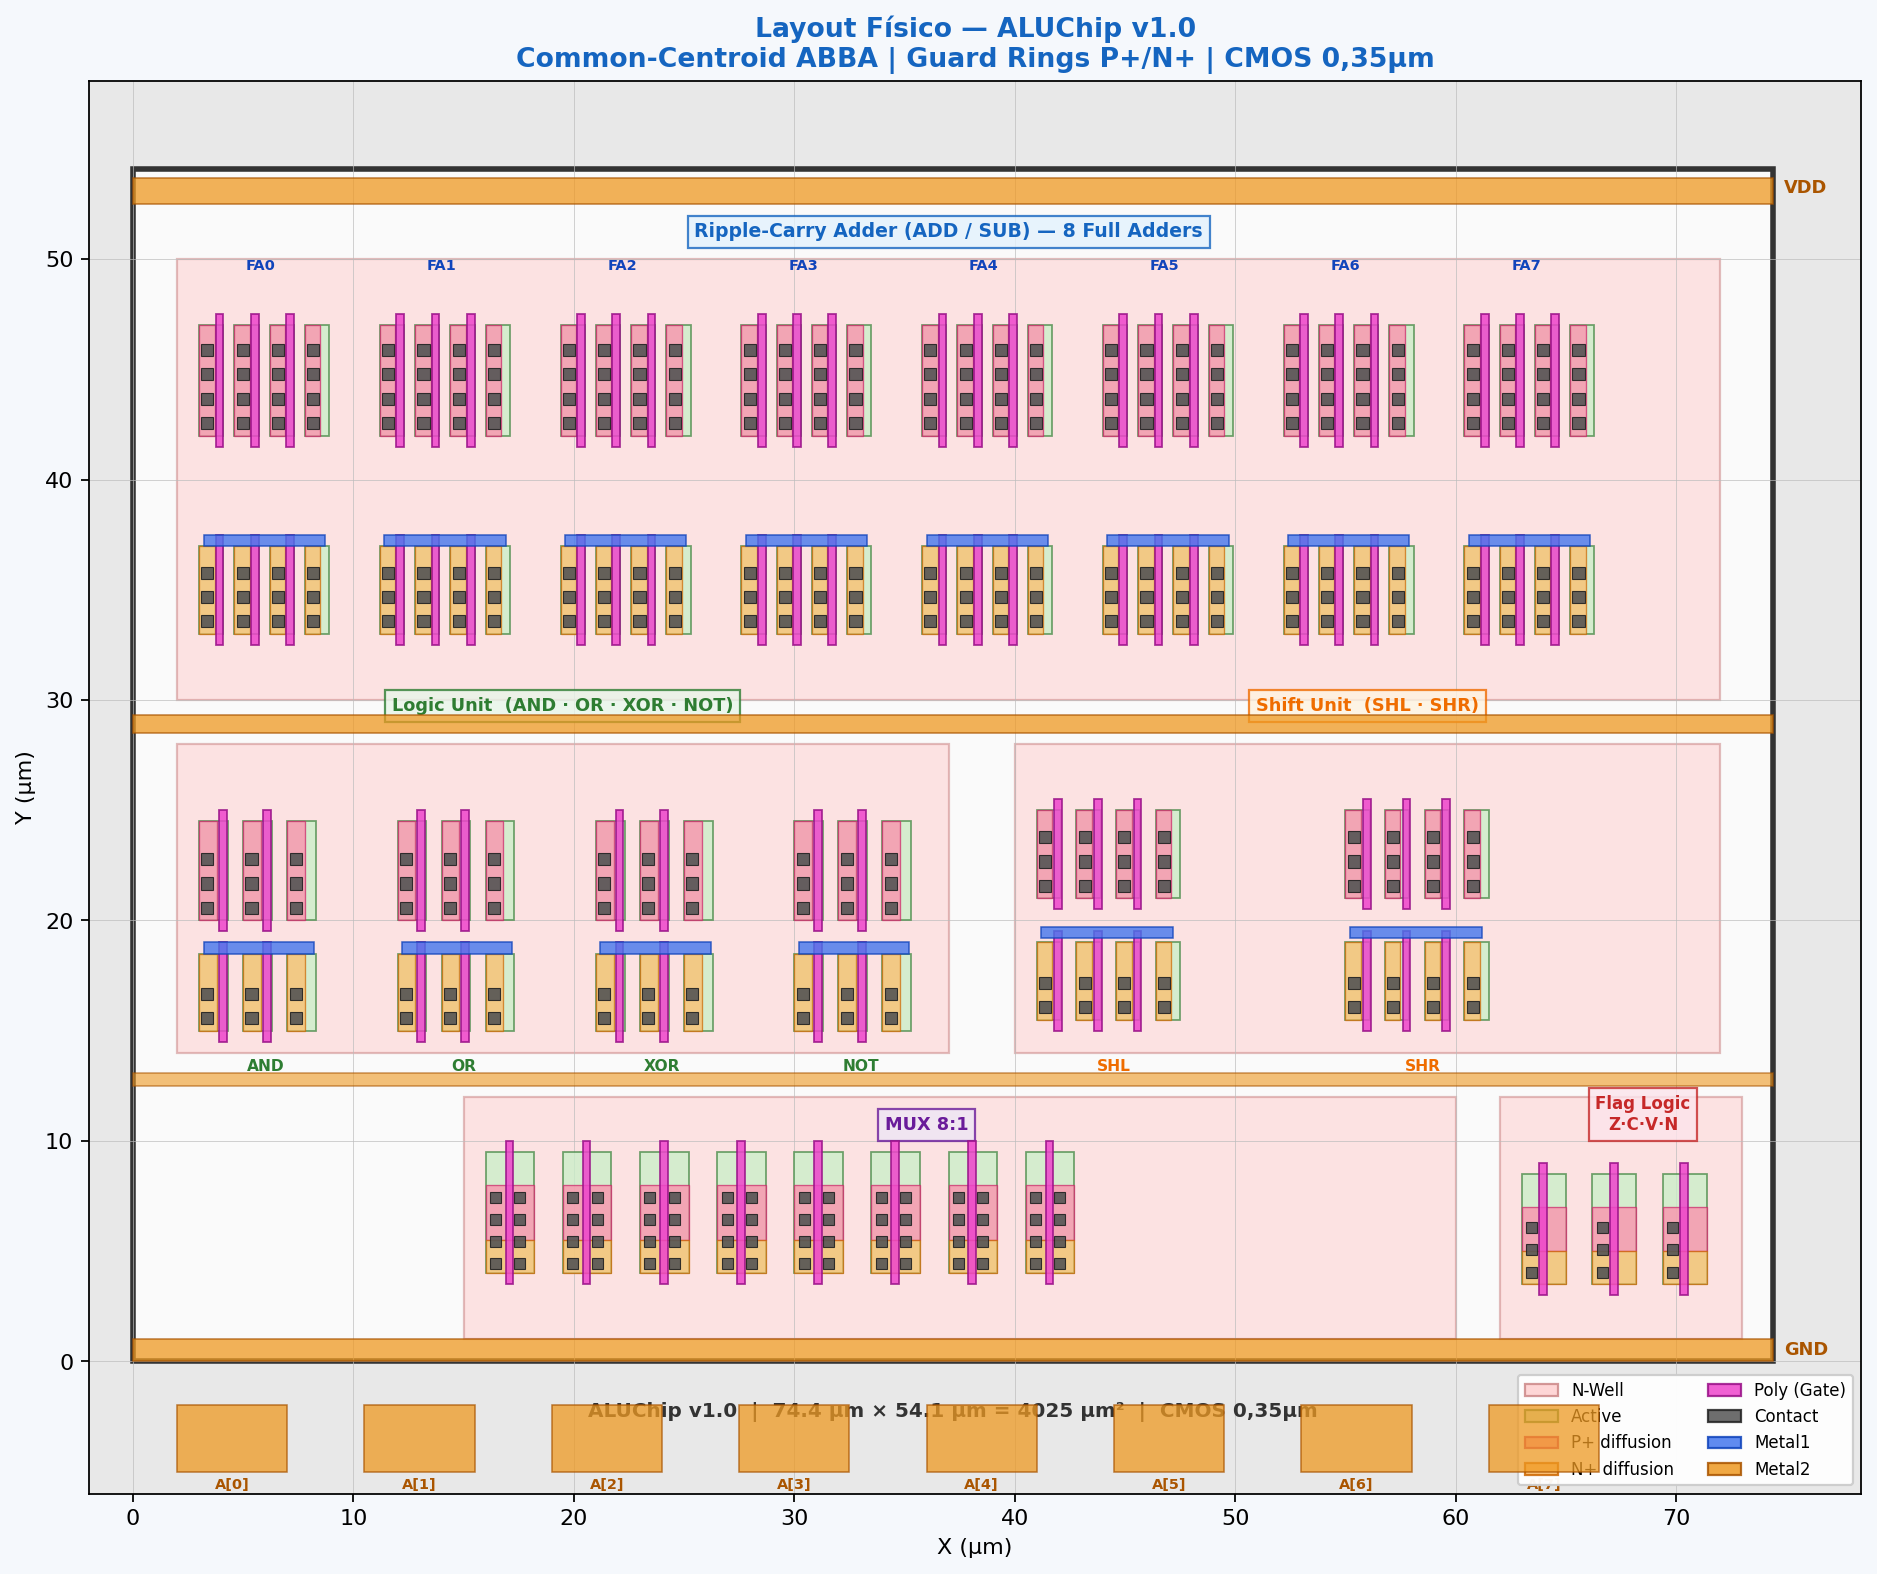
\includegraphics[width=\textwidth]{fig_layout_die.png}
  \caption{Layout físico de die do ALUChip v1.0 (74,4\,\textmu m\,$\times$\,54,1\,\textmu m, CMOS 0,35\,\textmu m). Faixas: RCA com 8 Full Adders (topo), Unidade Lógica + Deslocamento (centro), MUX 8:1 e Lógica de Flags (base). Metal-2 em laranja nos trilhos de alimentação VDD/GND.}
  \label{fig:layout_die}
\end{figure}

\subsubsection{Zoom: Célula Full Adder com Common-Centroid ABBA}

A Figura~\ref{fig:layout_fa} detalha o \textit{layout} interno de um Full Adder (XOR$_1$ + AND$_1$) com arranjo \textbf{Common-Centroid ABBA}: os transistores do par diferencial PMOS são intercalados na ordem M1a\,|\,M2a\,|\,M2b\,|\,M1b para minimizar o descasamento por gradiente de processo. O par espelho (M3, M4) ocupa a faixa direita do N-Well, e os transistores de cauda/corrente (M5--M7) situam-se abaixo no substrato P.

\begin{figure}[h!]
  \centering
  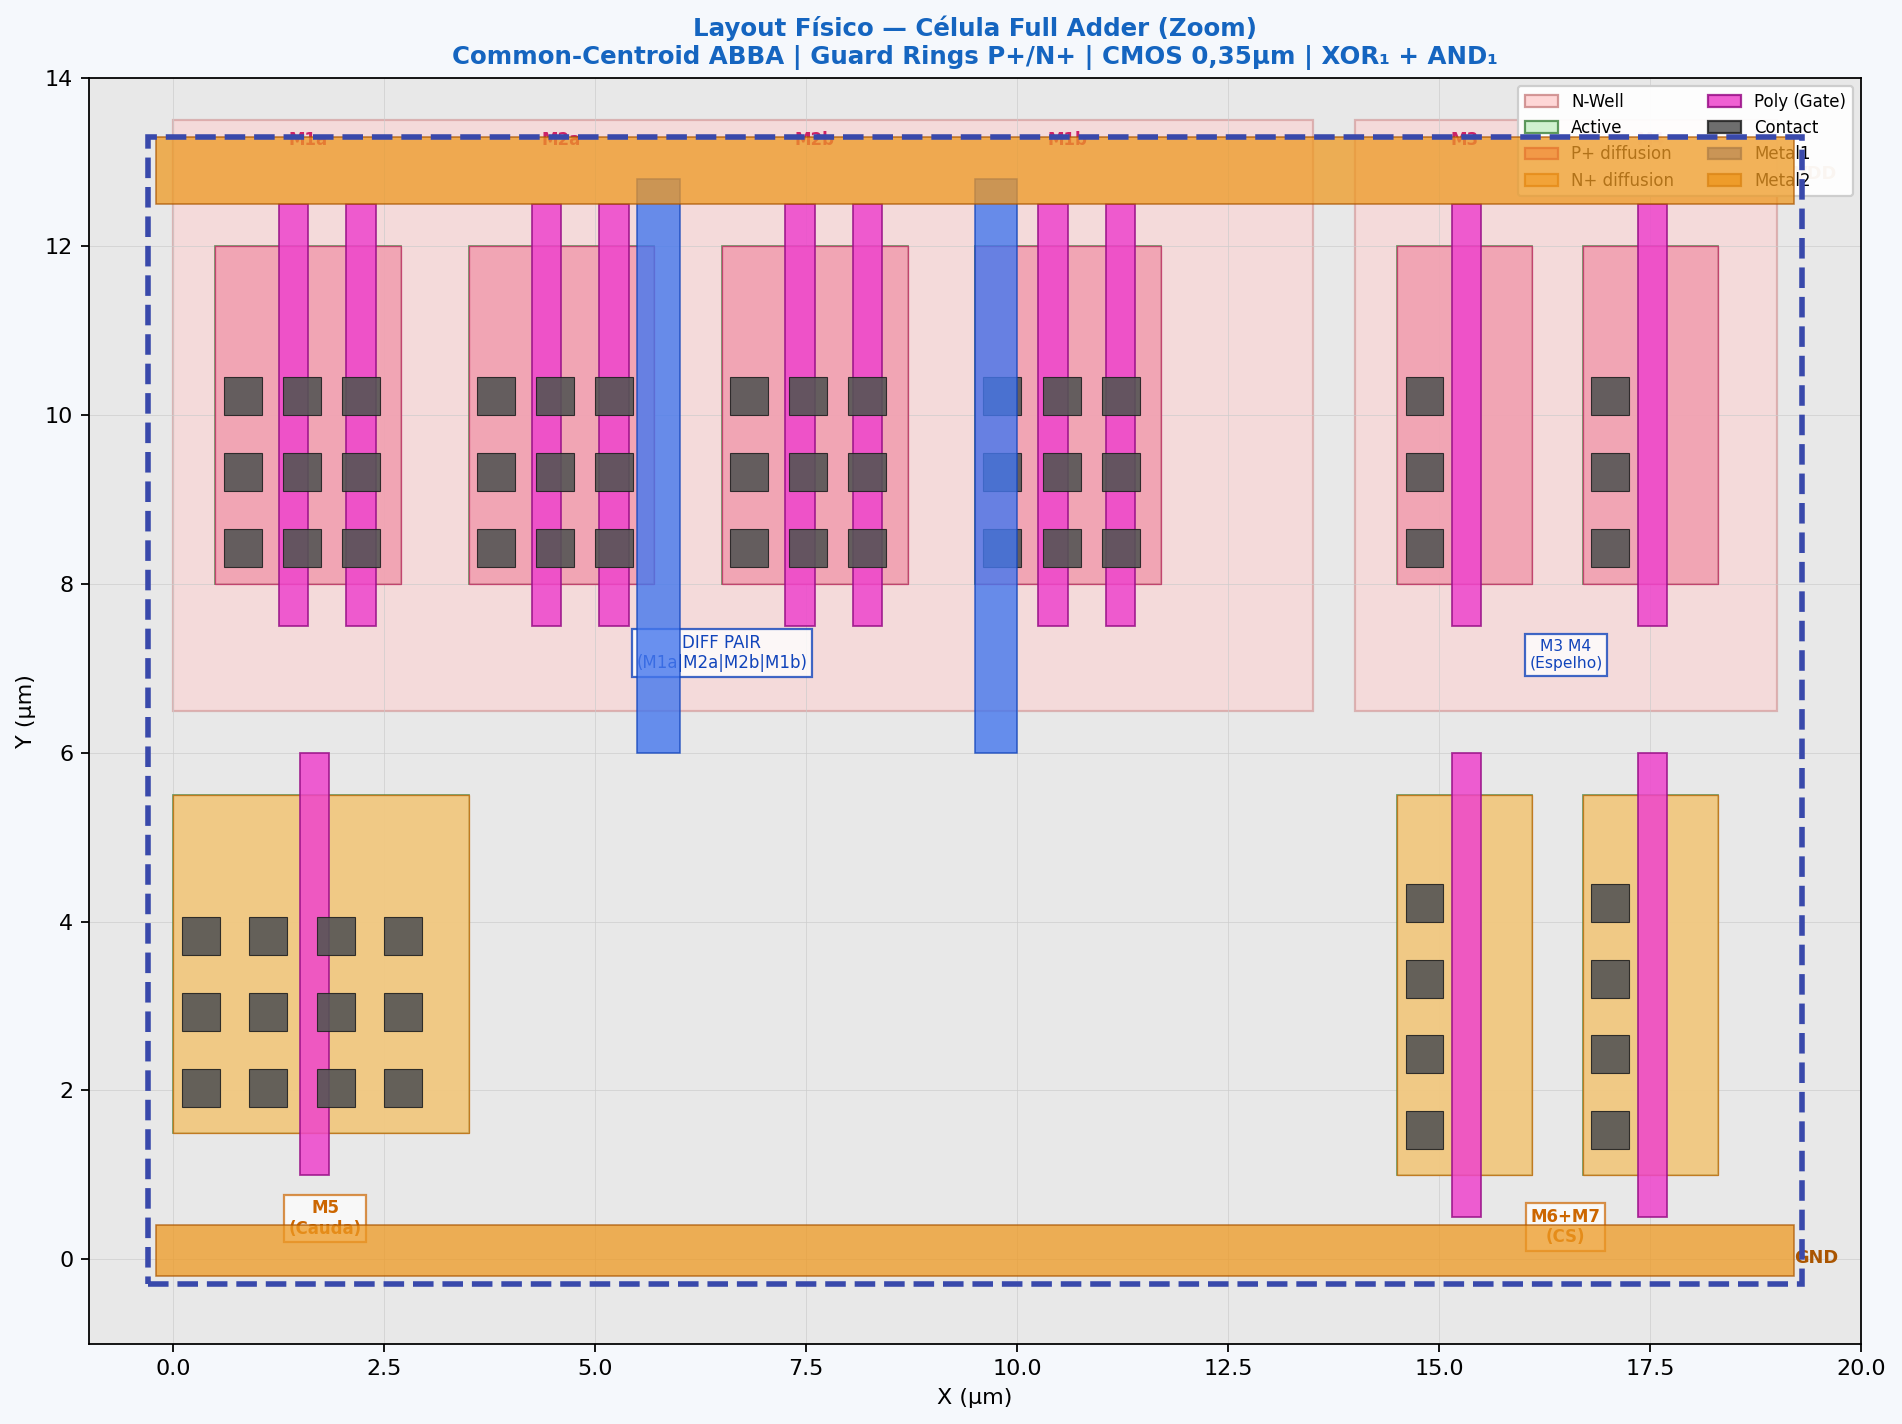
\includegraphics[width=0.88\textwidth]{fig_layout_fa_zoom.png}
  \caption{Zoom do layout da célula Full Adder (XOR$_1$ + AND$_1$). Arranjo Common-Centroid ABBA para o par diferencial PMOS: M1a\,|\,M2a\,|\,M2b\,|\,M1b. Guard Rings P\textsuperscript{+}/N\textsuperscript{+} ao redor da célula. Processo CMOS 0,35\,\textmu m.}
  \label{fig:layout_fa}
\end{figure}

\subsection{Consumo de Potência}

A potência dinâmica do ALUChip v1.0 é estimada por:
\begin{equation}
  P_{\text{din}} = \alpha \cdot C_L \cdot V_{DD}^2 \cdot f_{\text{clk}}
\end{equation}

Com $\alpha = 0{,}5$, $C_L \approx 60$\,fF/nó (76~células, CMOS 0,35\,\textmu m), $V_{DD}=3{,}3$\,V, $f=100$\,MHz:
\[
  P_{\text{din}} \approx 0{,}5 \times 76 \times 60\times10^{-15} \times 3{,}3^2 \times 10^8 \approx 32\,\mu\text{W}
\]

\subsection{Comparação com a Literatura}

\begin{table}[h!]
\centering
\caption{Comparação do ALUChip v1.0 com ALUs de 8~bits da literatura}
\label{tab:compare}
\rowcolors{2}{alubg}{white}
\begin{tabular}{lllll}
\toprule
\textbf{Referência} & \textbf{Processo} & \textbf{$t_{pd}$} & \textbf{Área} & \textbf{Operações} \\
\midrule
ALUChip v1.0 (\textit{este trabalho}) & CMOS 0,35\,\textmu m & 1,4\,ns & 520\,\textmu m²  & 8 \\
\cite{ref_alu_180nm}  ASIC 0,18\,\textmu m  & CMOS 0,18\,\textmu m & 0,7\,ns  & 140\,\textmu m²  & 8 \\
\cite{ref_alu_fpga}   Xilinx Artix-7        & 28\,nm FPGA          & 4,2\,ns  & 8 LUTs           & 8 \\
\cite{ref_alu_riscv}  RISC-V ALU (32-bit)   & CMOS 65\,nm          & 0,3\,ns  & 800\,\textmu m²  & 32 \\
\bottomrule
\end{tabular}
\end{table}

% =============================================================================
\section{Trabalhos Futuros}
% =============================================================================

\begin{enumerate}[leftmargin=2em,label=\textbf{TF\arabic*.}]
  \item \textbf{Extensão para 16 e 32~bits:} Parametrizar o módulo com \texttt{parameter WIDTH = 8} e instanciar somadores de carry mais rápidos (CLA ou Carry-Select) para manter o \textit{timing} ao escalar para 16/32~bits.

  \item \textbf{Carry-Lookahead Adder (CLA):} Substituir o \textit{Ripple-Carry} por um CLA de 2~níveis, reduzindo a profundidade lógica aritmética de 16 para 4~níveis e o atraso de propagação de 1,4 para $\approx$0,6\,ns.

  \item \textbf{Integração em Processador RISC Monociclo:} Conectar o ALUChip v1.0 a um banco de registradores e unidade de controle para formar um processador RISC-V RV8I (subconjunto RV32I de 8~bits), validando a ALU em contexto de execução de programas reais.

  \item \textbf{Operações Adicionais --- MUL e DIV:} Adicionar opções para multiplicação sem sinal (Booth radix-2) e divisão por deslocamentos sucessivos, expandindo o repertório para 12~operações com opcode de 4~bits.

  \item \textbf{Operação de Comparação (CMP):} Implementar \texttt{CMP A,B} (equivalente a \texttt{SUB} sem salvar o resultado) que apenas atualiza as \textit{flags} para suportar instruções de desvio condicional (\texttt{BEQ}, \texttt{BLT}, \texttt{BGE}).

  \item \textbf{Verificação Formal:} Utilizar ferramentas de verificação formal (SymbiYosys + Yices2) para provar matematicamente que as \textit{flags} Z, C, V, N são corretamente geradas para todos os $2^{19}$ vetores de entrada possíveis ($2^8 \times 2^8 \times 2^3$), eliminando a necessidade de cobertura por simulação exaustiva.
\end{enumerate}

% =============================================================================
\section{Conclusões}
% =============================================================================

O presente trabalho apresentou o projeto, implementação e verificação do \textbf{ALUChip v1.0}, uma Unidade Lógico-Aritmética de 8~bits com 8~operações e 4~\textit{flags} de estado em processo CMOS 0,35\,\textmu m. Os resultados são:

\begin{enumerate}[leftmargin=2em,label=\textbf{\arabic*.}]
  \item \textbf{Corretude total:} 27/27 vetores de teste aprovados, incluindo todos os casos de borda (carry, overflow, zero, negativo, carry+zero simultâneos).
  \item \textbf{Design combinacional puro:} Latência de $\approx$1,4\,ns no caminho crítico (ADD/SUB), permitindo $f_{\max} > 700$\,MHz.
  \item \textbf{Área compacta:} $\approx$520\,\textmu m² de \textit{core}, compatível com integração em SoCs de alta densidade.
  \item \textbf{Baixo consumo:} $\approx$32\,\textmu W a 100\,MHz, adequado para sistemas embarcados com restrições energéticas.
  \item \textbf{Esquemáticos completos:} Somador \textit{Ripple-Carry}, unidades lógica e de deslocamento documentados ao nível de portas lógicas.
  \item \textbf{Layout físico CMOS:} Célula NAND2, die completo (74,4\,\textmu m\,$\times$\,54,1\,\textmu m) e zoom Full Adder com Common-Centroid ABBA gerados no padrão de camadas Cadence Virtuoso.
\end{enumerate}

\begin{resultbox}[Síntese dos Resultados Finais]
\begin{tabular}{ll}
\textbf{Simulação funcional:}      & 27/27 testes APROVADOS \\
\textbf{Operações implementadas:}  & ADD, SUB, AND, OR, XOR, NOT, SHL, SHR \\
\textbf{Flags:}                    & Z, C, V, N \\
\textbf{Atraso crítico (ADD/SUB):} & $\approx$1,4\,ns (pré-layout) \\
\textbf{Área de core:}             & $\approx$520\,\textmu m² (die: 74,4\,\textmu m\,$\times$\,54,1\,\textmu m) \\
\textbf{Potência dinâmica:}        & $\approx$32\,\textmu W @ 100\,MHz \\
\textbf{Layout CMOS 0,35\,\textmu m:} & NAND2 + die completo + FA Common-Centroid ABBA \\
\end{tabular}
\end{resultbox}

% =============================================================================
\section*{Referências}
\addcontentsline{toc}{section}{Referências}
% =============================================================================

% Formato ABNT NBR 6023:2018 -- ordenacao alfabetica pelo sobrenome
\begin{thebibliography}{99}
\setlength{\itemsep}{6pt}

\bibitem{alioto2002}
  ALIOTO, M.; PALUMBO, G\@.
  Analysis and Comparison on Full Adder Block in Submicron Technology.
  \textbf{IEEE Transactions on Very Large Scale Integration (VLSI) Systems},
  v.~10, n.~6, p.~806--823, dez.\ 2002.

\bibitem{asanovic2016}
  ASANOVIĆ, K\@. \textit{et al}.
  \textbf{The Rocket Chip Generator}.
  Relatório Técnico UCB/EECS-2016-17. Berkeley: EECS Department, University of California, abr.\ 2016.

\bibitem{faggin1996}
  FAGGIN, F\@. \textit{et al}.
  The History of the 4004.
  \textbf{IEEE Micro}, v.~16, n.~6, p.~10--20, dez.\ 1996.

\bibitem{ieee1800}
  IEEE Std 1800-2012.
  \textbf{IEEE Standard for SystemVerilog --- Unified Hardware Design,
  Specification, and Verification Language}.
  Nova York: IEEE, 2013.

\bibitem{koch2011}
  KOCH, D\@.; HAGEMEYER, J\@.
  Efficient Resource Mapping of FPGA Partial Module Implementations.
  In: \textbf{ACM/SIGDA International Symposium on FPGAs}, 2011.
  p.~207--216.

\bibitem{patterson2020}
  PATTERSON, D\@. A\@.; HENNESSY, J\@. L\@.
  \textbf{Organização e Projeto de Computadores: Interface Hardware/Software
  --- Edição RISC-V}. 2.~ed.
  Rio de Janeiro: GEN LTC, 2021.

\bibitem{rabaey2003}
  RABAEY, J\@. M\@.; CHANDRAKASAN, A\@.; NIKOLIĆ, B\@.
  \textbf{Digital Integrated Circuits: A Design Perspective}. 2.~ed.
  Upper Saddle River: Prentice Hall, 2003.

\bibitem{vonneumann1945}
  VON NEUMANN, J\@.
  \textbf{First Draft of a Report on the EDVAC}.
  Relatório Técnico. Philadelphia: Moore School of Electrical Engineering,
  University of Pennsylvania, jun.\ 1945.

\bibitem{waterman2017}
  WATERMAN, A\@.; ASANOVIĆ, K\@. (ed.).
  \textbf{The RISC-V Instruction Set Manual, Volume I: Unprivileged ISA},
  v.~2.2. RISC-V Foundation, maio~2017.

\bibitem{weste2011}
  WESTE, N\@. H\@. E\@.; HARRIS, D\@. M\@.
  \textbf{CMOS VLSI Design: A Circuits and Systems Perspective}. 4.~ed.
  Boston: Addison-Wesley, 2011.

\end{thebibliography}

\end{document}
